%%%%%%%%%%%%%%%%%%%%%%%%%%%%%%%%%%%%%%%%
%% MCM/ICM LaTeX Template %%
%% 2021 MCM/ICM           %%
%%%%%%%%%%%%%%%%%%%%%%%%%%%%%%%%%%%%%%%%
\documentclass[12pt]{article}
\usepackage{geometry}
\geometry{left=1in,right=0.75in,top=1in,bottom=1in}

%%%%%%%%%%%%%%%%%%%%%%%%%%%%%%%%%%%%%%%%
% Replace ABCDEF in the next line with your chosen problem
% and replace 1111111 with your Team Control Number
\newcommand{\Problem}{C}
\newcommand{\Team}{2115921}
%%%%%%%%%%%%%%%%%%%%%%%%%%%%%%%%%%%%%%%%

\usepackage{newtxtext}
\usepackage{amsmath,amssymb,amsthm}
\usepackage{newtxmath} % must come after amsXXX

\usepackage{graphicx}
%\usepackage{xcolor}
\usepackage{fancyhdr}
\lhead{Team \Team}
\rhead{}
\cfoot{}

\newtheorem{theorem}{Theorem}
\newtheorem{corollary}[theorem]{Corollary}
\newtheorem{lemma}[theorem]{Lemma}
\newtheorem{definition}{Definition}

%%%%%%%%%%%%%%%%%%%%%%%%%%%%%%%%
%================================
\usepackage{enumerate}%\item 需要
\usepackage{tabularx}% \table 
\usepackage{booktabs}% 	\toprule
\usepackage{float}%图片浮动
\usepackage{graphicx}
\usepackage{bm}% reference
\usepackage{indentfirst} 
\setlength{\parindent}{2em} %2em代表首行缩进两个字符
\usepackage{listings}%代码
%================================
%\usepackage{color}
\usepackage[table]{xcolor}
\usepackage{colortbl}
\definecolor{mygray}{gray}{.9}
\definecolor{mypink}{rgb}{.99,.91,.95}
\definecolor{mycyan}{cmyk}{.3,0,0,0}
%===========================================

\begin{document}
	\setcounter{page}{1} 
	
%\graphicspath{{.}}  % Place your graphic files in the same directory as your main document
%\DeclareGraphicsExtensions{.pdf, .jpg, .tif, .png}
\thispagestyle{empty}
\vspace*{-16ex}
\centerline{\begin{tabular}{*3{c}}
	\parbox[t]{0.3\linewidth}{\begin{center}\textbf{Problem Chosen}\\ \Large \textcolor{red}{\Problem}\end{center}}
	& \parbox[t]{0.3\linewidth}{\begin{center}\textbf{2021\\ MCM/ICM\\ Summary Sheet}\end{center}}
	& \parbox[t]{0.3\linewidth}{\begin{center}\textbf{Team Control Number}\\ \Large \textcolor{red}{\Team}\end{center}}	\\
	\hline
\end{tabular}}

%==========================================
\renewcommand{\abstractname}{Summary}

%=====================================
%%%%%%%%%%% Begin Summary %%%%%%%%%%%
% Enter your summary here replacing the (red) text
% Replace the text from here ...

\begin{center}
	\large\textbf{  {A Hornet Relative Density Distribution model Based on Kernel Density Estimation and Xgboost Classifier
	}}
	\end{center}
\begin{abstract}
% and Report Credibility Prediction
To address the hornet-confirming challenge, we propose a species relative density distribution model based on \textbf{Kernel Density Estimation(KDE) Method}. KDE method can calculate the contribution of all samples to the density function at each space position (the decay mode of density contribution with distance is determined by and kernel function), so as to calculate the density distribution function of species in the whole space.  We estimate the uncertainty level of the prediction at location $X$ by the density of report beside $X$ since the denser the samples in the vicinity of X, the more accurate the prediction of the model. This results of this method is proved to be intuitive and robust by experiments.

To predict the species distribution over time, we devide the whole timespan into several time windows and propose a updated strategy synthesizing the historical distribution and new report information in the current time window. The length of the time window is just how often we update the model. Minimum appropriate time window length is determined by whether enough reports is received within the time window.

We then built a \textbf{Xgboost classifier} for unverified reports prediction. Feature like the month the report occurred, description about the bee is extracted. What's more, \textbf{image classification algorithm based on EfficientNet} and \textbf{ Sentiment Classification algorithm based on BERT} are used to dig information from images dataset, witness' description and laboratory comments. In order to solve the imbalance of image samples, data enhancement and \textbf{Focal Loss} functions were used to effectively adjust the process of image preprocessing and CNN training. However, suffered from severe data imbalance, Xgboost classifier performs poorly. Therefore, we make the choice to use the species distribution function which is independent of unverified report prediction.

Based on model established above, we propose a report priorities model and set up conditions to determine whether hornet species has been eradicated.

To assess report priorities, both the \textbf{uncertainty level of report's location} and the \textbf{predicted credibility} of report itself are taken into account.

The \textbf{eradication} of hornets can be defined as the maximum value of its relative density function is less than a certain threshold.

Our framework shows a strong robustness. The species relative density estimation model doesn't depend on meshing the space and provides a continuous prediction. Metrics of our species relative density distribution model is stable with regard to manually given parameter.

\textbf{Keywords}: KDE-method, Species Density Estimation, EfficientNet, Xgboost classifier

\end{abstract}
% to here
%%%%%%%%%%% End Summary %%%%%%%%%%%

%%%%%%%%%%%%%%%%%%%%%%%%%%%%%%
\clearpage
\pagestyle{fancy}
% Uncomment the next line to generate a Table of Contents
\rhead{Page \thepage\ of 23}
\tableofcontents 
\newpage

%%%%%%%%%%%%%%%%%%%%%%%%%%%%%%


\section{Introduction}
\subsection{Problem Background}
The nest of the scientific name Vespa mandarinia was discovered on Vancouver Island in British Columbia, Canada, in September 2019. The nest was quickly destroyed, but the news of the incident spread quickly across the area. Since then, there have been several confirmed sightings of vermin in the neighboring state of Washington, as well as many false sightings. Researchers need to effectively identify the most likely species identification among reports so that they can effectively document and predict the path of species spread.

\subsection{Problems to be solved}
Here are the problems to be solved:
\begin{enumerate}[\quad\bf1.]
	\item We should build a model to predict the \textbf{geographic distribution} of hornets; Explain \textbf{the method and how often this model is updated} when new reports are received.
	\item We should build a binary classifier to predict \textbf{how likely a report is to be positive};
	\item We should build a model to evaluate the \textbf{Priority Level} of unverified sightings.To guide the government agencies about which reports should be investigated first.
	\item We should gave \textbf{conditions} under which we could prove that hornet species had \textbf{disappeared for studied area}.
\end{enumerate}

\section{Preparation of the Models}

\subsection{Assumptions}
To simplify our model and eliminate the complexity, we make the following main assumptions in this literature. All assumptions will be re-emphasized once they are used in the construction of our model:
\begin{enumerate}[\bfseries 1.]
	\item The spread of this pest over time can be described by a ground truth probability function $f^*(x,y,t)$, it is the proportion of established hornets in all bees at position $(x,y)$ and time $t$. However, with limited information we can only get a estimation $\mu(x,y,t)$ with variance $\sigma(x,y,t)$.
	\item $f(x,y,t)$ may lacks special structure but it is continuous, that would make it easy to optimize. $f$ is derivative-free(evaluations do not give gradient information).
	\item Government agencies has limited resource and verify a report can be costly. Therefore, evaluating $f$ is expensive and the number of times we can evaluate it is severely limited. The purpose of carrying out a investigation is to make the estimation of $f$ as accurate as possible.
	\item Unverified report can also povide information about the probability of hornet activity. The estimated probability $p(info)$ can be extracted by pictures, descriptions and other information.
\end{enumerate}
\subsection{Notations}
In this work, we use the nomenclature in  \textbf{Table \ref{Ntt}} in the model construction. Other nonefrequent-used symbols will be introduced once they are used.

\begin{table}[H]
	\begin{center}
		\caption{Notations}
		\begin{tabular}{cl}
			\toprule
			\multicolumn{1}{m{3cm}}{\centering Symbol}
			&\multicolumn{1}{m{8cm}}{\centering Definition}\\
			\midrule
			$X=(x,y),t$&The longitude, latitude and time\\
			$f^*(X,t)$&The ground truth probability function that hornets are present\\
			$\hat{\mu}_i(X,t)$&The estimation of $f^*(X,t)$ based on new report in ith time window\\
			${\mu}_i(X,t)$&The estimation of $f^*(X,t)$ based on new report in ith time window\\
			$\sigma_i(X,t)$&The Uncertainty Level of relative density prediction at position $X$\\
			$p_i$&The Unverified Report Credibility\\
			\bottomrule
		\end{tabular}\label{Ntt}
	\end{center}
\end{table}

\subsection{Data Filtration and Abnormal Value Processing}
Since the major subject of our study is the spread of hornets, time is a key variable. Therefore, report without valid date is worthless. We drop reports whose 'Detection Date' is '<Null>' or before 2000 year. Moreover, report before 2010 is so sparse that not every year there's a new report. So we drop reports before 2010. Then we plot the density function for the rest of the data as is shown in {Figure \ref{report_kde}}.
\begin{figure}[H]%\usepackage{float}
	\small
	\centering
	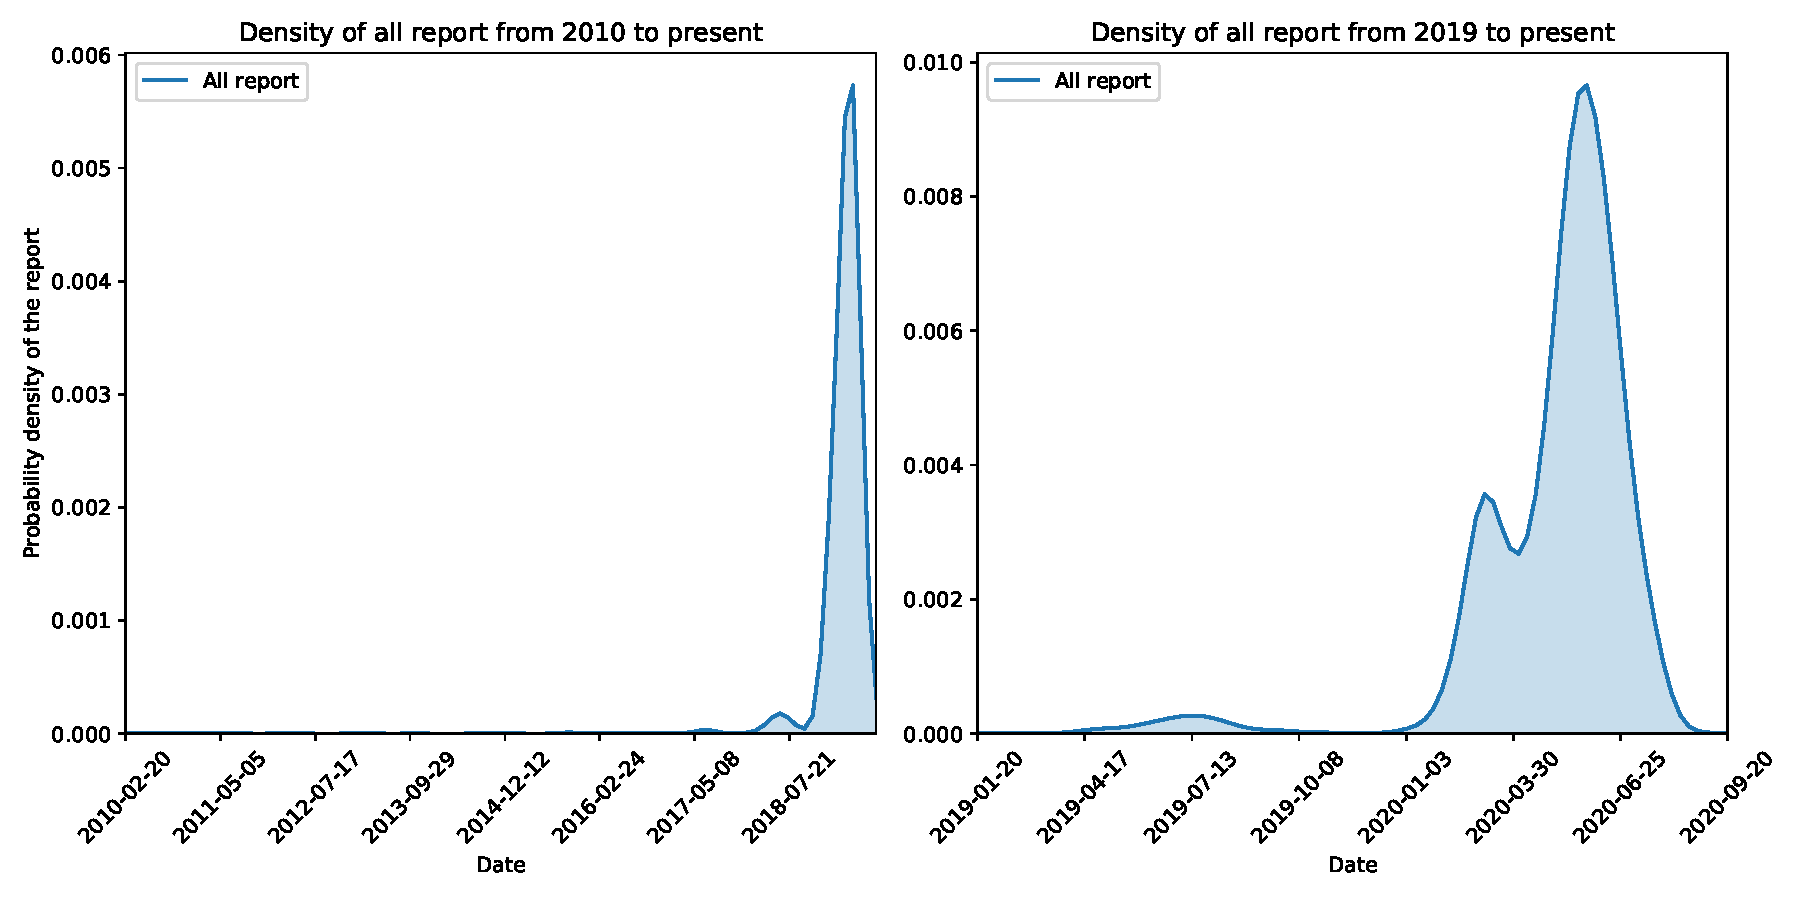
\includegraphics[width=17cm]{./pictures/report_kdes}
	\caption{Distribution of all report over time}\label{report_kde}
\end{figure}
According to {Figure \ref{report_kde}}, proportion of reports before May 2019 is negligible. Therefore our research focus on reports from 2019-5 to present. {Figure \ref{report_bar}} shows the number of reports in  each Lab Status and in each month. Obviously this is a highly unbalanced data set for more than 96\% reports is negative.
\begin{figure}[!htbp]
	\small
	\centering
	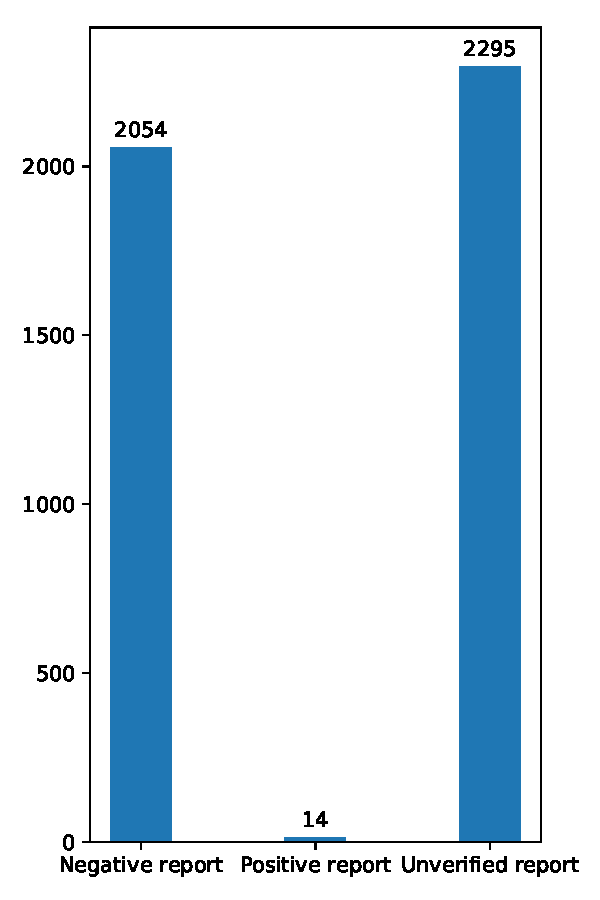
\includegraphics[width=5cm]{./pictures/class_bar.pdf}
	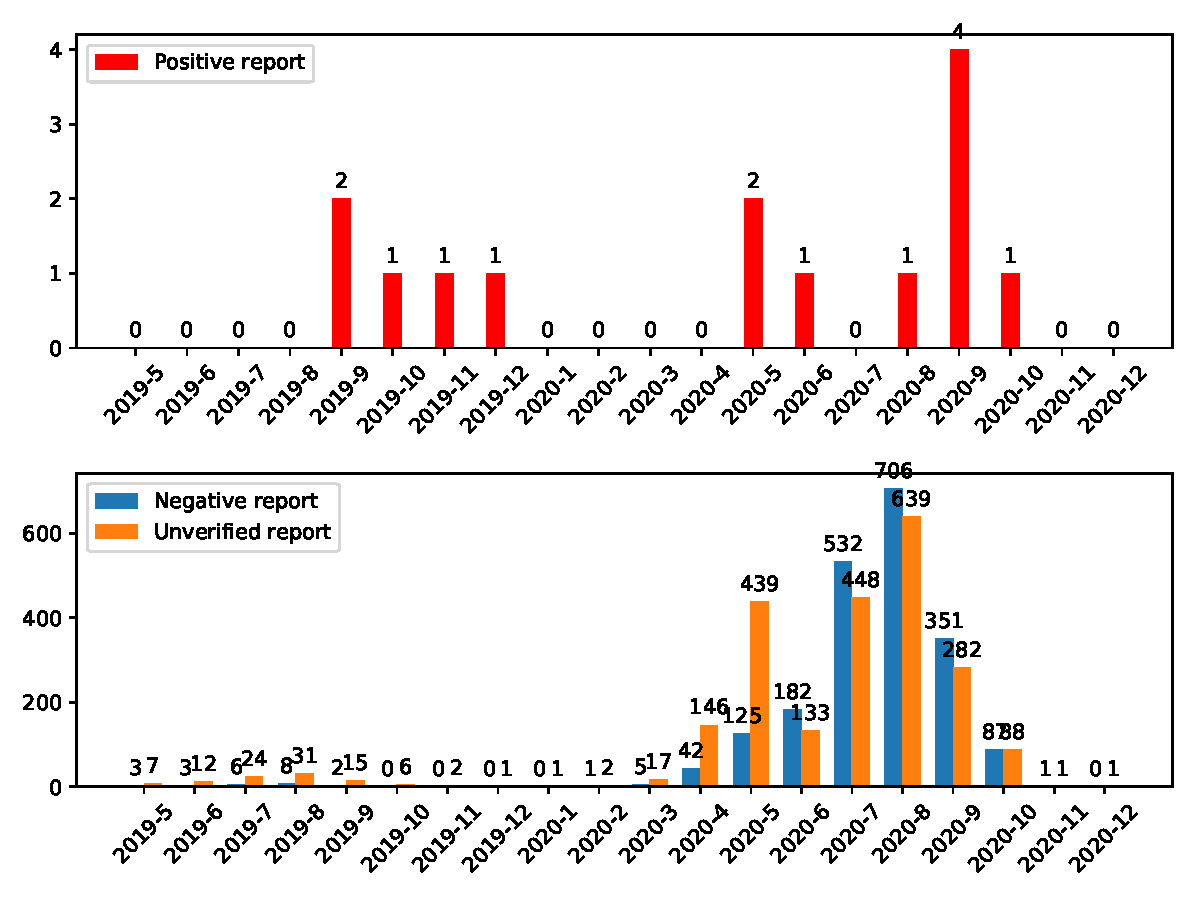
\includegraphics[width=10cm]{./pictures/report_bar.pdf}
	\caption{Distribution of all report over Lab Status and month}\label{report_bar}
\end{figure}


\section{Model Construction}
\subsection{Quantitative description of hornets distribution}
\subsubsection{Model building}
Predicting the spread of hornets can be seen as a presence-only modeling of species distributions. Many methods have been used for such purpose. Generalized linear models (GLMs) and generalized
additive models (GAMs) is widely used from species distribution to environmental management\cite{GLMs}.  A Bayesian approach \cite{Bayesian} proposed modeling presence versus a random
sample. ENFA, Hirzel et al proposed Environmental-Niche Factor Analysis using presence localities together with environmental data for the study area\cite{Ecological‐niche}.


Our method modeling species’ geographic distributions is \textbf{Kernel Density Estimation Method} (\textbf{KDE-Method})\cite{1}. In our data set, additional environmental data is not provided and available geographic information of reports is just longitude and latitude. KDE-Method is suitable for modeling spacial disctance and can output a distribution function estimating species density.

Unlike histograms, kernel estimators are smooth and does not depend on the width of the bins and the end points of the bins. Kernel estimators smooth out the contribution of each data point over a local neighbourhood of that data point. The contribution of data point $X_i$ to the estimate at some point $X$ depends on the  between $X_i$ and $X$ are.The extent of this contribution is dependent upon the shape of the kernel function adopted and the width (bandwidth) accorded to it. If we denote the kernel function as K and its bandwidth by h, the estimated density at any point $X$ is

\begin{equation}
\hat{{f}}(X)=\frac{1}{n}\sum_{i=1}^{n}K\left(X, X_i\right),
\end{equation}
where $\int K(t)dt=1$ to ensure that the estimates  integrates to 1. $X$ is a position vector. The kernel function $K$ is usually chosen to be a smooth unimodal function with a peak at 0. RBF kernel is one of the most widely used kernels due to its similarity to the Gaussian distribution. This kernel can be mathematically represented as
\begin{equation}
	K\left(X, X'\right)=\exp(-\gamma \|X-X'\|^2),
	\label{gamma}
\end{equation}
where $\gamma $ is a positive parameter.

We use Python API \textbf{sklearn.svm.OneClassSVM} in to solve the kernel density. \textbf{Figure \ref{species_svm}} shows the kernel density of all reports since 2019-5 and the parameter $\gamma =3$.
\begin{figure}[H]%\usepackage{float}
	\small
	\centering
	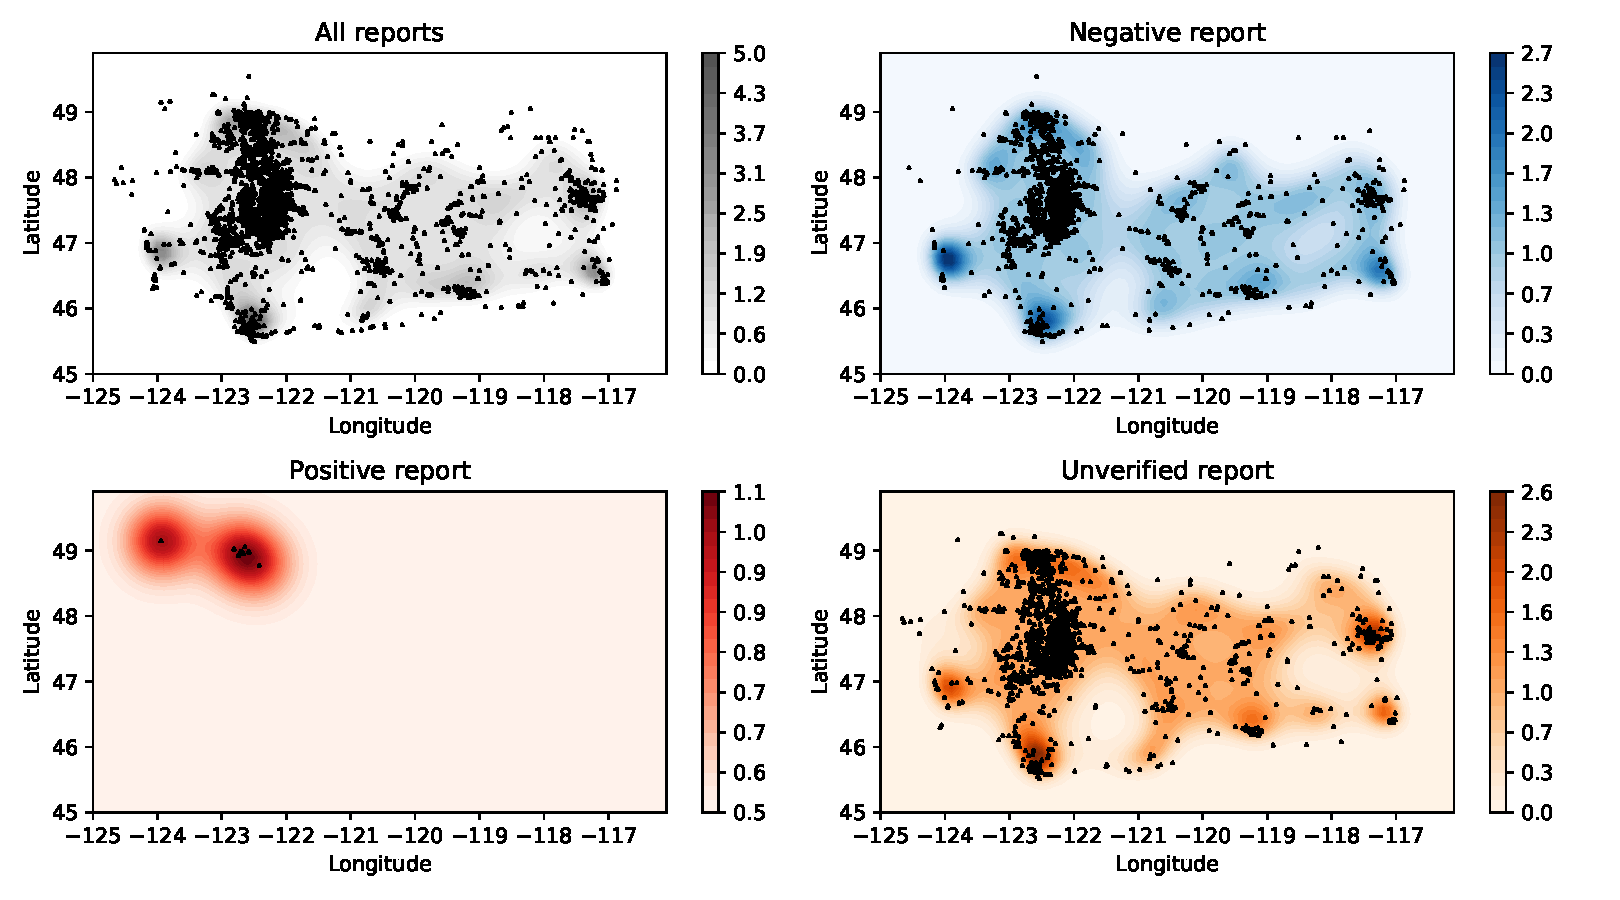
\includegraphics[width=17cm]{./pictures/species_svm}
	\caption{The Kernel Density of All Reports since 2019-5}\label{species_svm}
\end{figure}

To describe the spread process of hornets, we split all the reports by date in time window of 30 days. Then we estimate the kernel density of positive and negative reports represented as:
\begin{equation}
	\hat{f}(X, t, \Delta t, label)=\frac{1}{n}\sum_{X_i\in S(t, label)}K\left(X, X_i\right),
\end{equation}
where $label=0,1,2$ represents \textbf{negative, positive and unverified} report respectively.  $S(t, \Delta t, label)$ represents set of all reports with time window of length $\Delta t$ after time $t$ and has \textbf{Lab Comments} corresponding to $label$. $n$ is the size of $S(t, \Delta t, label)$.

Intuitively, the proportion of established hornets in all bees is the ratio of density of positive and negative reports.
\begin{equation}
	\hat{\mu}(X, t, \Delta t) = \frac{\hat{{f}}(X, t, \Delta t, 1)}{\hat{{f}}(X, t, \Delta t, 0)+\hat{{f}}(X, t, \Delta t, 1)}
	\label{mu1}
\end{equation}

According to \textbf{Equation \ref{mu1}} unverified report does not have any contribution to $\mu $. But in fact, we can build a model to infer how likely an unverified report is to be a positive example. This model take image file, notes and lab comments as input, probability as output denoted as 
\begin{equation}
	p_i=p(Image_i, Note_i, LabComment_i).
\end{equation} If $p_i$ is available, $\hat{\mu}$ can be corrected to be 
	
\begin{equation}
	\hat{\mu}(X, t, \Delta t) = \frac{\hat{{f}}(X, t, \Delta t, 1)+\frac{1}{n}\sum_{X_i\in S(t, label)}p_iK\left(X, X_i\right)}{\hat{{f}}(X, t, \Delta t, 0)+\hat{{f}}(X, t, \Delta t, 1)+\hat{{f}}(X, t, \Delta t, 2)}
	\label{mu}
\end{equation}

The 'hat' sign on $\mu $ indicates that $\hat{\mu}$ only depends on reports within time window $(t, t+\Delta t)$ and does not take former reports into consideration. However, it is reasonable to assume that a part of hornets which have been recorded before still inhabit in the original area. Therefore, final estimation $\mu$ take both former estimation and new reports into consideration. $\mu_i(X)$ represents the proportion of established hornets at position $X$ in ith time window.

\begin{equation}
	\mu_i(X) =\frac{w \cdot \mu_{i-1}(X) +  \hat{\mu_i}(X)}{w+1} , i=1,2,...,n
	\label{nu_update}
\end{equation}
where the $n$ is the number of time windows the whole timespan is devided into. $w$ is the weight of the historical information.
$\mu_i(X)$ measures the distribution of hornets over a period of time. \textbf{Figure \ref{species_spread_svm_10}} shows the sequence $\mu_i(X)$ estimated by \textbf{Equation \ref{mu1}} with $w=0.5$. It can visually show the spread of hornets over time.

\begin{figure}[H]%\usepackage{float}
	\small
	\centering
	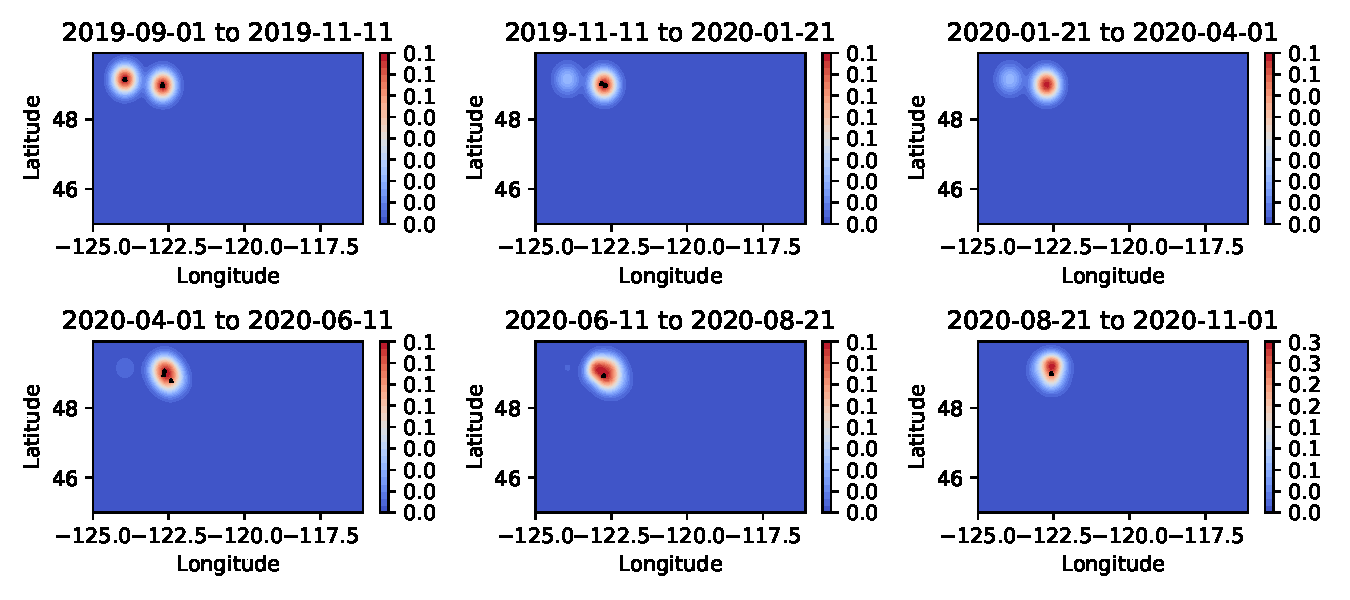
\includegraphics[width=17cm]{./pictures/species_spread_svm_10}
	\caption{$\mu_i(X)$ since 2019-9 with $\gamma=7, w=1$}\label{species_spread_svm_10}
\end{figure}


Since the report received is only the partial sampling of the actual species distribution, $\mu(X, t)$ has  a certain amount of uncertainty $\sigma(X, t)$. The more spatially dense the samples are, the more accurate the estimation of the density function will be. The uncertainty level of $\mu(X, t)$ can be defined as 
\begin{equation}
	\sigma(X, t, \Delta t) = \exp (-\hat{{f}}(X, t, \Delta t, 0)-\hat{{f}}(X, t, \Delta t, 1)).
	\label{uncertainty}
\end{equation}
$\sigma_i(X) \approx 1$ means that the samples near $X$ in ith time window is so sparse that we are completely unsure of the density estimate.

\subsubsection{Model evaluation}
model performance using receiver operating characteristic(ROC) curves. ROC analysis was developed in signal processing and is widely used in clinical medicine\cite{roc}. The main advantage of ROC analysis is that area under the ROC curve (AUC) provides a single measure of model performance, independent of any particular choice of threshold.\cite{2} 

By definition, species relative density distribution function $\mu_i(X)$ is the proportion of established hornets in all bees. It can be seen as the probability of a report at position $X$ to be positive output by our model.
We evaluate the model by mean ROC of a 5-fold cross-validation. For the positive report is sparse in both time and space. We evaluate the model on a long timespan from 2019-09 to 2020-11. Parameter setting is $\gamma=7$ and for we only have 1 time window, $w$ dosn't matter.
\textbf{Figure \ref{species_3d_mu}} shows comparison between species density $\hat{f}_i(X, 1), \hat{f}_i(X, 0) $ and hornets' relative density distribution $\mu_i(X)$

\begin{figure}[H]%\usepackage{float}
	\small
	\centering
	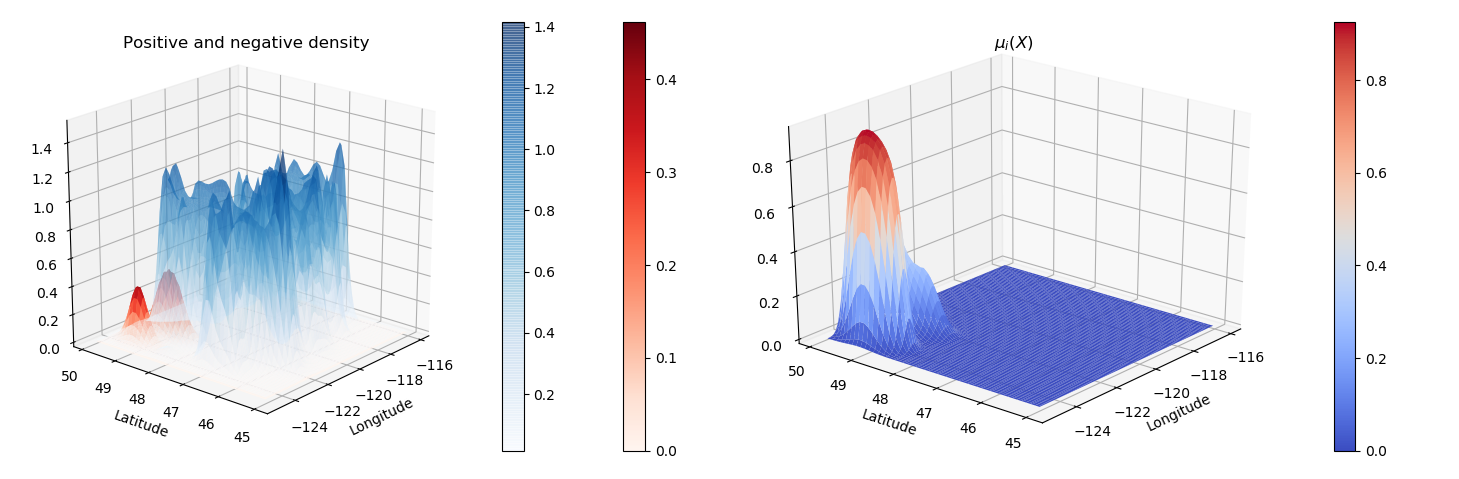
\includegraphics[width=17cm]{./pictures/species_3d_mu.png}
	\caption{Positive and negative density and $\mu_i(X)$ with $\gamma=7$}\label{species_3d_mu}
\end{figure}

\textbf{Figure \ref{species_total_mu_roc}} shows $\mu_i(X)$ and ROC curve of our model. The mean area under the ROC curve (AUC) is 0.75 which provides a level of precision of our species distribution model.

\begin{figure}[H]%\usepackage{float}
	\small
	\centering
	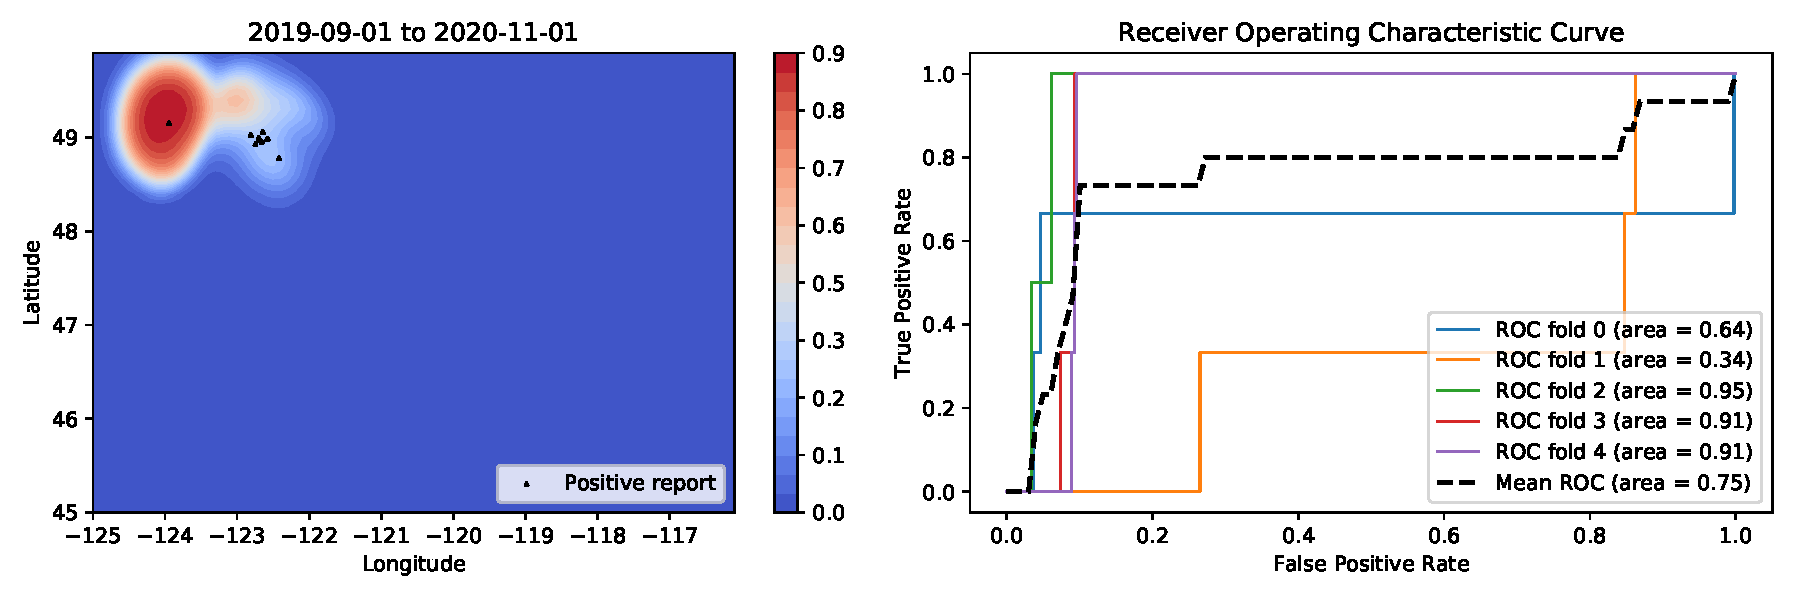
\includegraphics[width=17cm]{./pictures/species_total_mu_roc.pdf}
	\caption{$\mu_i(X)$ and ROC curve with $\gamma=7$}\label{species_total_mu_roc}
\end{figure}


\subsection{EfficientNet Convolutional Neural Network for Image Classification}
When it comes to image classification problem, we usually use Convolutional Neural Network to train a model to help us.Efficientnet is a popular neural network that can take into account both the speed and accuracy of the model, making it faster and more efficient for image processing tasks.

\subsubsection{Low Quality Image Filtering}
Before using EfficientNet for training, we can see that in some of the images, the part of bee is so indistinct that it is impossible to distinguish any of the detailed features of the bee. It's hard for a neural network to learn anything about the difference between a hornets and a normal bee from these pictures. Therefore, before training, we need to get rid of these low quality pictures.

We use three image classification networks vgg16, resnet50 and mobilenet pretrained on Imagenet\cite{Imagenet} as picture filter. ImageNet uses a list of 1000 non-overlapping classes, including bees. ImageNet can be applied in object recognition, image classification and automatic object clustering. For each input image, our picture filter give a confidence probability for all 1000 classes. 

Intuitively, the more bee features in the image, the greater the confidence probability of the CNN network output bee class. 
Therefore we can evaluate the image quality by the minimum confidence probability that the input image is classified as bee. Then we can manually choose a threshold $p_t$ and drop images whose quality is lower than the threshold. In our experiments we found that the model does perform better to classify the hornet species using filtered image dataset.

\subsubsection{Classification Target and Evaluation}
A convolutional neural network $\mathcal{N}$ can be represented by the whole convolution  layers
\begin{equation}
\mathcal{N}=\mathcal{F}_{k} \odot \ldots \odot \mathcal{F}_{2} \odot =  \mathcal{F}_{1}\left(X_{1}\right)
\end{equation}

In fact, multiple convolutional layers with the same structure are usually referred to as a stage. The convolutional layer structure in each stage is the same (except the first layer is a downsampling layer). The convolutional layer can be convolved in the unit of stage. Network $\mathcal{N}$ is expressed as:

\begin{equation}
%\odot_{j=1 \ldots k} \mathcal{F}_{j}\left(X_{1}\right)\underset{i=1 \ldots s}{\bullet}%
\mathcal{N}= \odot_{j=1 \ldots s} \mathcal{F}_{i}^{L_{i}}\left(X_{\left\langle H_{i}, W_{i}, C_{i}\right\rangle}\right)
\end{equation}
and $< H_i,W_i,C_i>$ represents the dimensions of the  $i$th input tensor,$i$ (from 1 to $s$) represents the sequence number of the stage $\mathcal{F}_{i}^{L_{i}}$ represents the $i$th stage It consists of a convolutional layer $ F_{i}$ repeated $L_{i}$ times.

we change the output dimensions into 2 class numbers reprensents the prediction label of hornet species $ Y = \{ \hat p_0,\hat p_1 \} $ then we choose the max possibility of $P$.
After we have received the predicted hornet label, we can get four statistical  metrics.

\begin{itemize}
	\item[1] TP(True Positive):The true value is positive and the model considers the number positive 
	\item[2] FN(False Negative):The true value is positive and the model considers that the number is negative 
	\item[3] FP(False Positive):The true value is negative, the number considered positive by the model 
	\item[4] TN(True Negative):The true value is negative, and the model considers the number negative.
\end{itemize}

we can use the Confusion Matrix and $F_1$ score to choose the best model for image classfication.

\begin{equation}
	 \begin{cases}
	\mathcal{N}& =\odot_{j=1 \ldots s} \mathcal{F}_{i}^{L_{i}}\left(X_{\left\langle H_{i}, W_{i}, C_{i}\right\rangle}\right) \\
	Y& =\mathcal{N}(X_1) \\
	\hat y &  =\mathop{\arg\min Y} \\
	P & = \frac{TP}{TP+FP} \\
	R & = \frac{TP}{TP+FP} \\
	Accuracy& =\frac{\mathrm{TP}+\mathrm{TN}}{\mathrm{TP}+\mathrm{TN}+\mathrm{FP}+\mathrm{FN}} \\
	F_1 &= \frac{2 \times P \times R}{P+R}
	\end{cases}
\end{equation}
 
	

%(1)Population migrationd is.
%
%b.Variables

%\begin{table}[H]
%	\centering
%	\caption{ four method}\label{y}
%	\begin{tabularx}{0.9\textwidth}{cllll}
%		\toprule
%		method  & total precision  & Pacific Wren & Hermit Thrush&Varied Thrush \\
%		\midrule
%		Bayes & 50  & 100 & 16.67& 0 \\
%		\rowcolor{mygray}
%		K-Nearest Neighbors  & 29.94  &50 & 16.67 & 16.67  \\
%		Kernel SVM  & 36.84   & 12.5 & 16.67 &0 \\
%		\rowcolor{mygray}
%		Logistic Regression  & 52.63  & 62.5 & 16.67 &0 \\
%		
%		\bottomrule
%	
%\end{tabularx}
%\end{table}
\subsubsection{EfficientNet Structure}
EfficientNet\cite{EfficientNet} provides a new model scaling approach is used for an effective network. To extend the network from depth, width and resolution, it utilizes a simple and powerful composite coefficient. It does not arbitrarily scale the dimensions of the network like the conventional approach. The optimum group of parameters (composite coefficient) can be obtained based on the neural structure search technology. Not only is EfficientNet much faster than other networks, it also has greater accuracy.

\begin{figure}[H]
	\small
	\centering
	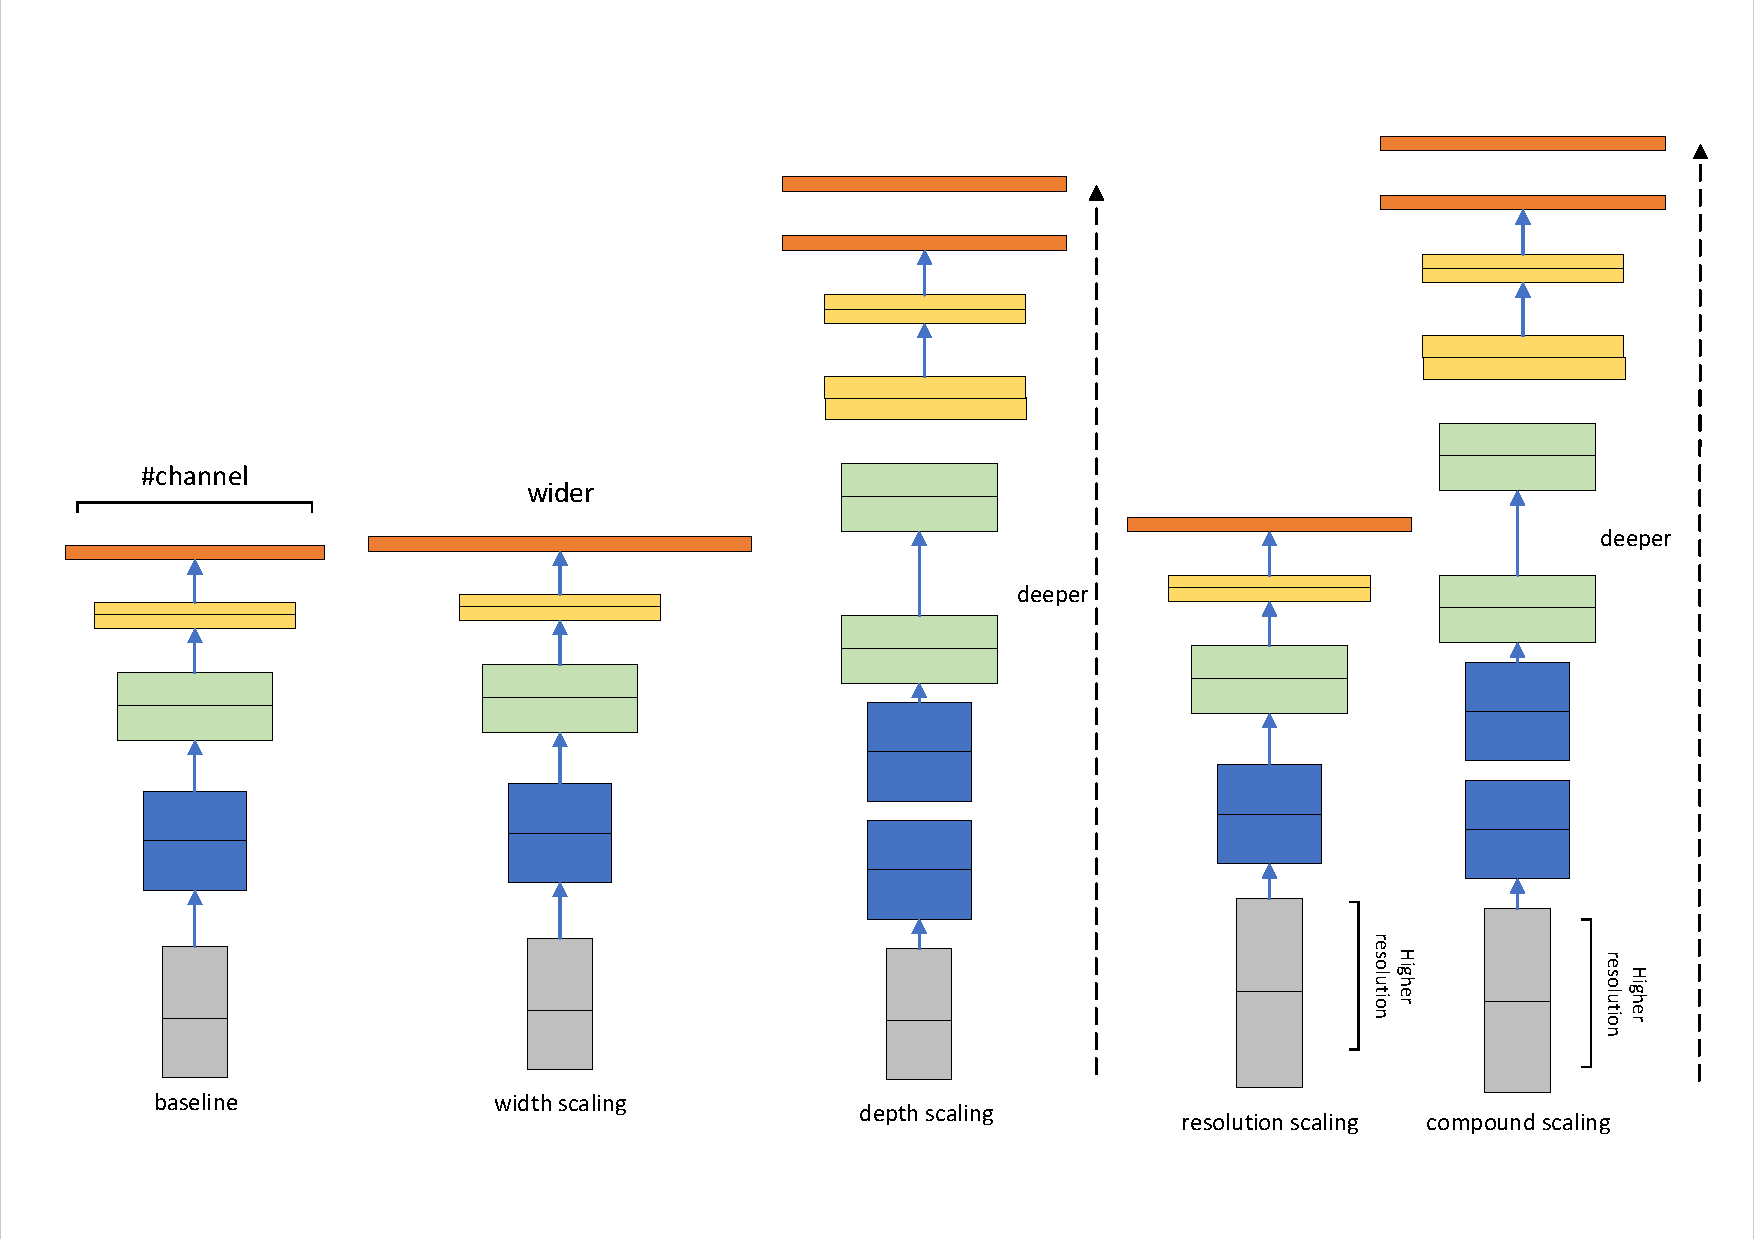
\includegraphics[width=14cm]{./pictures/network_scale.pdf}
	\caption{EfficientNet scales technology}\label{jj}
\end{figure}



\begin{table}[H]
	\centering
	\caption{ EfficientNet-B0 baseline network}\label{y}
	\begin{tabularx}{0.9\textwidth}{clllllllll}
		\toprule
%		Stage & Operators & Resolution & Channels  &Varied Layers  \\
		Stage $i$ & Operator $\hat {\mathcal{F}}_{i}$ & Resolution $\hat H_{i} \times \hat W_{i}$ & Channels $\hat C_{i}$ &Varied Layers $\hat L_{i}$  \\
		\midrule
		1 & Conv3x3  &  $224 \times 224$ & 32& 1 \\
		\rowcolor{mygray}
		2 & MBConv1,k3x3  & $112 \times 112$ & 16& 1\\
		3 & MBConv6,k3x3  & $112 \times 112$  &24& 2 \\
		\rowcolor{mygray}
		4 & MBConv6,k5x5 &$56 \times 56$& 40& 2\\
		5 & MBConv6,k3x3  & $28 \times 28$ & 80& 3 \\
		\rowcolor{mygray}
		6 & MBConv6,k5x5 &$14 \times 14$ & 112& 3 \\
		7 & MBConv6,k5x5 & $14 \times 14$  & 192& 4 \\
		\rowcolor{mygray}
		8 & MBConv6,k3x3  &  $7 \times 7$ & 320& 1 \\
		9 & Conv1x1,Pooling,FC  &$7 \times 7$  &1280& 1 \\
		\bottomrule
	\end{tabularx}
\end{table}	

In EfficientNet, a compound expansion method is proposed. $\alpha,\beta,\gamma$ a set of parameters that we need to solve, and the optimal parameter with constraints is solved. They measure the proportions of depth, width, and resolution respectively. $\beta,\gamma$ have a Square constraint, because if you increase the width or resolution twice, the amount of calculation will increase by four times, but if you increase the depth twice, the amount of calculation Will be doubled. 
\begin{equation}
\begin{array}{l}
\text { depth: } d=\alpha^{\phi} \\
\text { width: } w=\beta^{\phi} \\
\text { resolution: } r=\gamma^{\phi} \\
\text { s.t. } \alpha \cdot \beta^{2} \cdot \gamma^{2} \approx 2 \\
\alpha \geq 1, \beta \geq 1, \gamma \geq 1
\end{array}
\end{equation}

The calculation amount of convolution operation (FLOPS) is proportional to $d , \beta^{2}, \gamma^{2}$ We can adjust the hyper-parameters $\phi$Under this constraint, after $\phi$ is specified, the calculation amount of the network will be approximately $2^\phi$ times the previous .

Therefore, our network calculations can be controlled under the specified hyperparameters $\phi$. The model will affect the with depth resolution of the network through the adjustment of other parameters, and find the best parameters in the grid search.

\subsubsection{Focal Loss Function}
There are only 14 positive samples, which is less than one-tenth of the negative samples. Our image data is extremely unbalanced. The traditional cross-entropy loss function cannot effectively solve this problem. Data filtering is only a partial solution to the problem of sample imbalance as is shown in \textbf{Figure \ref{Classes_Imbalance}}. Except for the case of $p_0>0.6$, the selected images are still at least 5 times larger than the original positive samples, and there are 3 samples in the positive examples that are useless, so we only have 10 valid positive samples. 

\begin{figure}[H]%\usepackage{float}
	\small
	\centering
	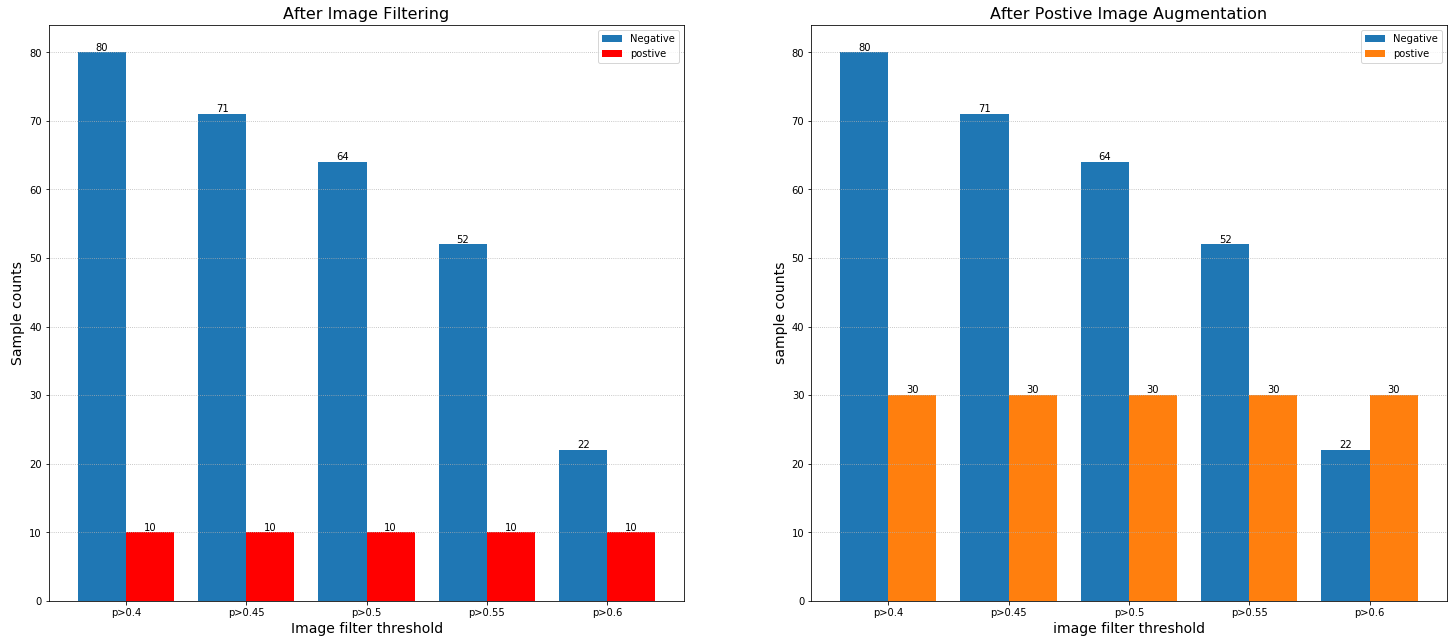
\includegraphics[width=17cm]{./pictures/Classes_Imbalance.png}
	\caption{Data filtering can partialy solve class imbalance}\label{Classes_Imbalance}
\end{figure}
We hope to further solve the problem of sample imbalance by modifying the loss function. \textbf{Focal loss} has been proved effective to calibrate deep neural network\cite{focal_loss}. We introduce the focal loss starting from the cross entropy (CE) loss for binary classification.

\begin{equation}
\operatorname{CE}(p, y)=\left\{\begin{array}{ll}
-\log (p) & \text { if } y=1 \\
-\log (1-p) & \text { otherwise }
\end{array}\right.
\end{equation}

In the above $y \in \{ \pm1 \}$ specifies the ground-truth class and
$p \in \left[ 0,1 \right]  $is the model’s estimated probability for the class
with label $y = 1$. For notational convenience, we define $p_t$:
\begin{equation}
p_{\mathrm{t}}=\left\{\begin{array}{ll}
p & \text { if } y=1 \\
1-p & \text { otherwise }
\end{array}\right.
\end{equation}
and rewrite $\mathrm{CE}(p, y)=\mathrm{CE}\left(p_{\mathrm{t}}\right)=-\log \left(p_{\mathrm{t}}\right)$

in order to reshape the loss function to down-weight easy examples and thus focus training on hard negatives.we can add a modulating factor
$(1 - p_t)^{\gamma}$ to the cross entropy loss, with tunable focusing parameter $\gamma \geq 0$ . We define the focal loss as:

\begin{equation}
\mathrm{FL}\left(p_{\mathrm{t}}\right)=-\left(1-p_{\mathrm{t}}\right)^{\gamma} \log \left(p_{\mathrm{t}}\right)
\end{equation}



\subsubsection{K-fold Cross Validation}
Due to the small number of samples and imbalance, we should use K-Fold cross-validation\cite{k_fold_cv} to split the image dataset. Because there are too few positive samples in the data set, cross validation can make the evaluation to the performance of the model trained under certain hyperparameters more accurate. Furthermore, we can adjust k in different values to find the best k value for our datasets maximizing the performance of the network. 

Ariginal data is devided into K groups (K-Fold), makes a validation set for each subset of data, and uses the remaining K-1 subset of data as the training datasets, so that K models will be obtained. The K models are evaluated in the validation dataset,then use an average loss and accuracy for model evaluating.



% \begin{figure}[H]%\usepackage{float}
% 	\small
% 	\centering
% 	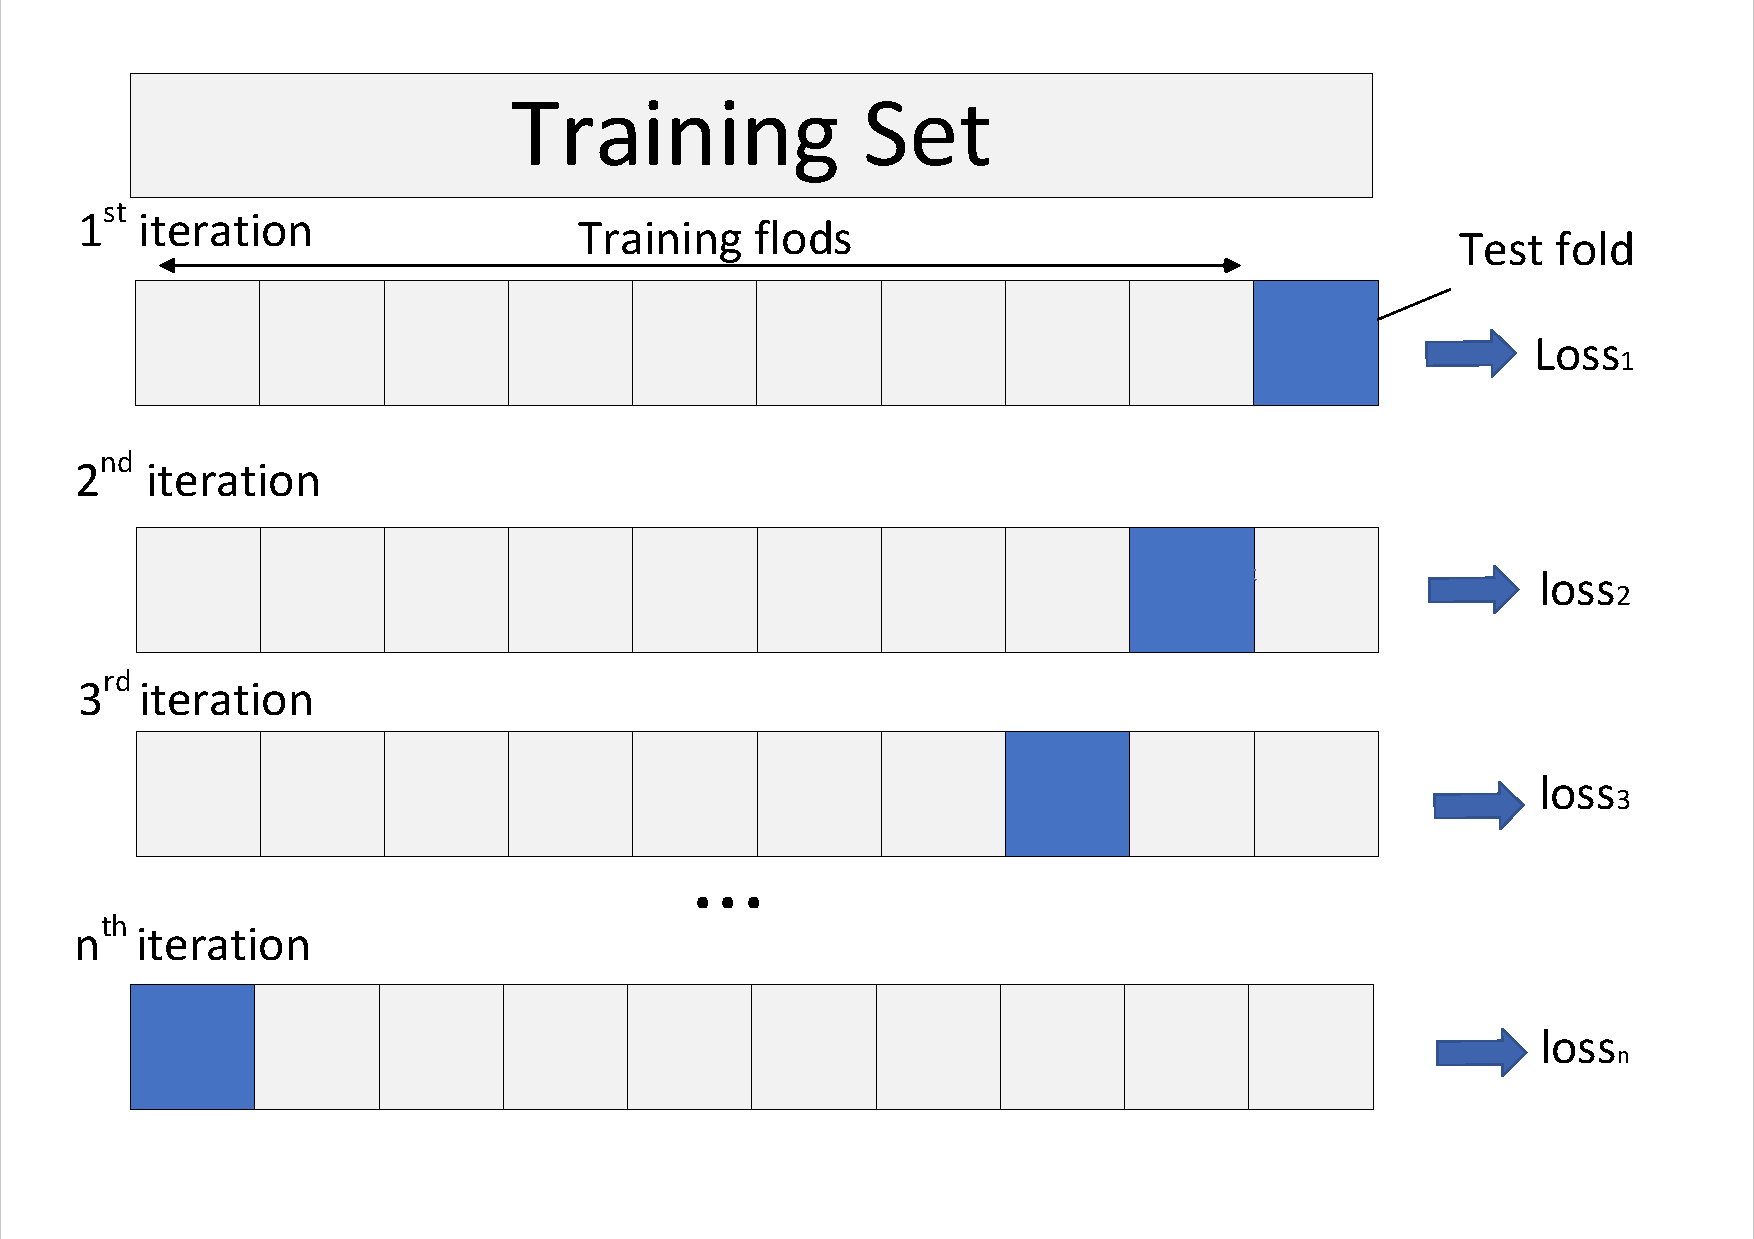
\includegraphics[width=14cm]{./pictures/kflod_grapgh.pdf}
% 	\caption{K-Fold Cross Validation}\label{jj}
% \end{figure}

\begin{equation}
\mathrm{Loss}_{(n)}=\frac{1}{n} \sum_{i=1}^{n} \mathrm{Loss}_{i}
\end{equation}

\begin{equation}
macro-P=\frac{1}{n} \sum_{i=1}^{n} P_{i}
\end{equation}

\begin{equation}
macro-R=\frac{1}{n} \sum_{i=1}^{n} R_{i}
\end{equation}

\begin{equation}
macro-{F_1} = \frac{2 \times macro-P \times macro-R}{macro-P+macro-R}
\end{equation}

We select different k values, perform multiple test experiments on the data, and extract the various metrics of each fold, and calculate their average value,then we can choose the best k for our datasets.

\subsubsection{Result and analysis}
After many tests, we found that when k=10 and the threshold of p0 is set to 0.5, the effect is the best, and when fold=2, we obtain the best model effect, and give his various metrics and Confusion matrix.
\begin{table}[H]
	\centering
	\caption{Metrics of the best model}\label{y}
	\begin{tabularx}{0.45\textwidth}{clll}
		\toprule
		 metrics & value &  metrics & value  \\
		%	Stage $i$ & Operator $\hat \mathcal{F}_{i}$ & Resolution $\hat H_{i} \times \hat W_{i}$ & Channels $\hat C_{i}$ &Varied Layers $\hat L_{i}$  \\
		\midrule
		Recall & 0.8850  &  Precision & 0.8403\\
		Accuracy & 0.7434 & $F_1$ & 16\\
		\bottomrule
	\end{tabularx}
\end{table}	


% Table generated by Excel2LaTeX from sheet 'Sheet1'
\begin{table}[htbp]
	\centering
	\caption{Positive Predicticon for Unverified image of the best model}
	  \begin{tabular}{lr}
	  \toprule
	  GlobalID & \multicolumn{1}{l}{possibility} \\
	  \midrule
	  {882EC093-D907-454C-A9EE-8D1DC46A4291} & 0.535679 \\
	  \rowcolor{mygray}
	  {05F3D0A6-EAC3-472F-A591-D2D21D7A91B2} & 0.659352 \\
	  {9A5CB940-8951-4FE7-8619-DAF4A8FE1850} & 0.599529 \\
	  \rowcolor{mygray}
	  {D8F21BBA-7ED8-41EE-B068-1C2030580FBD} & 0.503856 \\
	  {13B67BCB-AFCE-4100-AD2B-76EF178BA228} & 0.543146 \\
	  \rowcolor{mygray}
	  {B95A5C78-19CE-4C75-8763-1A8BB952F141} & 0.573015 \\
	  {98D817B8-BB8B-4C31-9A42-DEED4491599C} & 0.58357 \\
	  \rowcolor{mygray}
	  {BBBA5BA0-CAFB-43D3-8F1D-FB2D9CF777E0} & 0.756872 \\
	  \bottomrule
	  \end{tabular}%
	\label{Positive_Predicticon}%
  \end{table}%
  
\begin{figure}[H]%\usepackage{float}
	\small
	\centering
	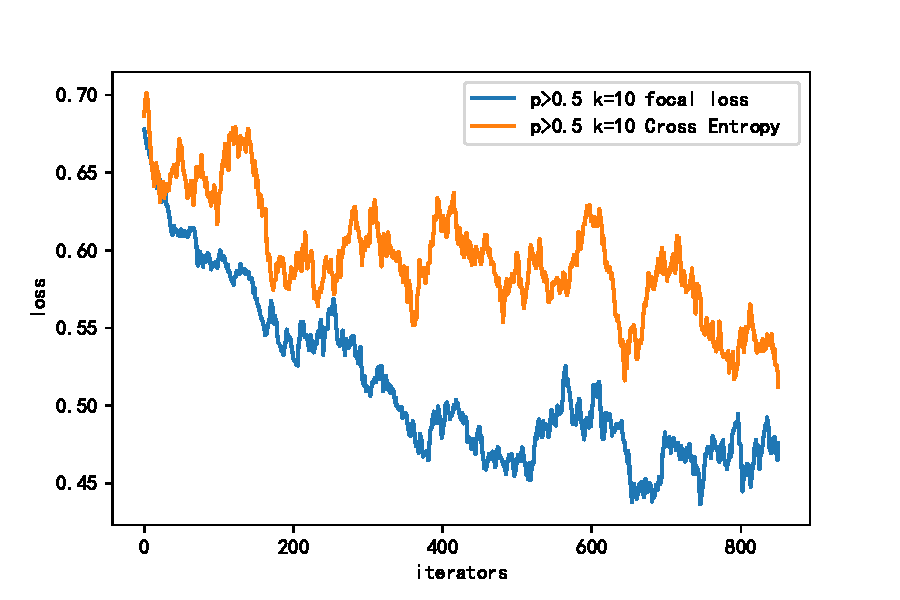
\includegraphics[width=8.5cm]{./pictures/focal_loss}
	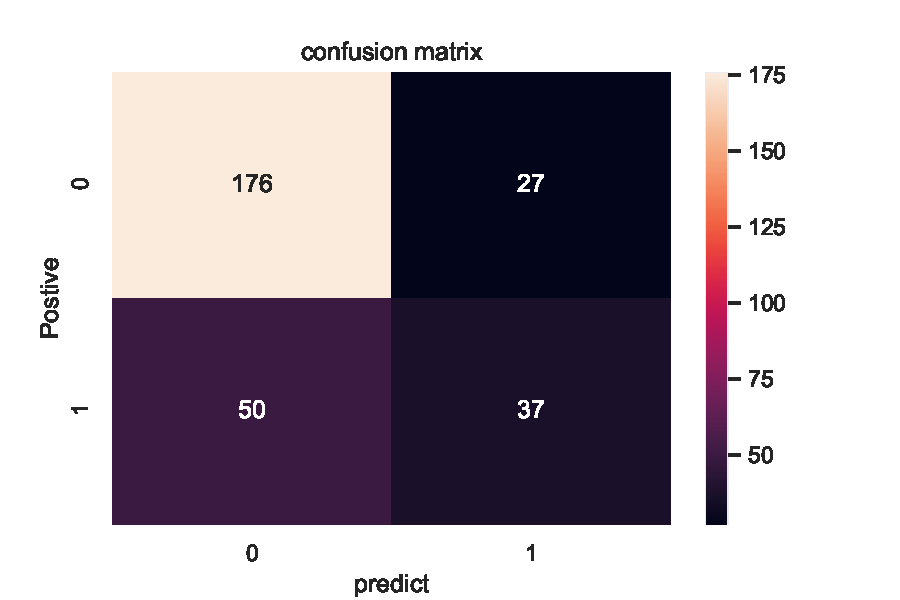
\includegraphics[width=8.5cm]{./pictures/confusion_matrix}
	\caption{Training Loss and Confusion Matrix of the best model}\label{confusion_matrix}
\end{figure}

\subsection{Unverified Report Prediction}
\subsubsection{Feature Engineering}
We first perform feature engineering on the dataset. The predicted results of the EfficientNet is used as a feature. Due to the life habits of the hornet are related to the month. We take the month of the sighting date as a feature. Then we looked at how to extract information from eyewitness' description and laboratory comments.

The hornet's length and color is a distinguishing feature compared to other bees. But because of the different eyewitness' description way. It is difficult to extract information directly representing the characteristics of bees from the text.So let's simplify the problem.As long as the bee's length and color are mentioned in the sighting report, we assume that the eyewitness was deeply impressed by the length and color of the bees in the sighting which suggests that the sighting is more likely to be positive. Therefore, whether the words related to length and color appear or not is extracted as a binary feature. Also, we assume that the length of the report also reflects the credibility of the report to some extent.

Laboratory reviews are the responses that experts give to witnesses after reading information about the reports. The strength of its positive emotions may reflect the credibility of the report in one way. We use pretrained \textbf{FINBERT}\cite{sentiment_analysis}, a language model based on BERT\cite{BERT}, as the sentiment analysis model. 

For missing values, we simply fill them in with zero.

\textbf{Table \ref{tab:examples}} includes few examples' engineered feature.
% Table generated by Excel2LaTeX from sheet 'final'
\begin{table}[htbp]
	\centering
	\caption{Few examples of our dataset after feature engineering}
	  \begin{tabular}{rrrrrrrr}
	  \toprule
	  \multicolumn{1}{l}{lenth} & \multicolumn{1}{l}{note sentiment} & \multicolumn{1}{l}{lab sentiment} & \multicolumn{1}{l}{color} & \multicolumn{1}{l}{bee lenth} & \multicolumn{1}{l}{EfficientNet pred} & \multicolumn{1}{l}{Season} & \multicolumn{1}{l}{Lab Status} \\
	  \midrule
	  0.00  & 0.00  & 0.04  & 0     & 0     & 0.58  & 6     & 1 \\
	  \rowcolor{mygray}
	  0.00  & 0.00  & 0.09  & 0     & 0     & 0.73  & 6     & 1 \\
	  0.70  & 0.06  & 0.07  & 1     & 1     & 0.54  & 7     & 0 \\
	  \rowcolor{mygray}
	  0.42  & 0.41  & 0.22  & 0     & 1     & 0.63  & 7     & 0 \\
	  0.30  & 0.07  & 0.10  & 0     & 1     & 0.76  & 6     & 0 \\
	  \bottomrule
	  \end{tabular}%
	\label{tab:examples}%
  \end{table}%
  
  
\subsubsection{Xgboost Classification Model}

The idea behind XGBoost's multi-classifier system is to build a decision tree in a gradient way, and then iterate gradually, adding a tree in each iteration and adjusting it so that it can reduce the current prediction error, gradually forming a strong evaluator integrating multiple tree models\cite{Xgboost}.

We use Python API \textbf{xgboost.XGBClassifier} to build the classifier with hyperparameter specified by \textbf{Table \ref{tab:Xgboost_hyperparameter}} .
% Table generated by Excel2LaTeX from sheet 'Sheet1'
\begin{table}[htbp]
	\centering
	\caption{hyperparameter of Xgboost classifier}
	  \begin{tabular}{ll}
	  \toprule
	  hyperparameter  & \multicolumn{1}{l}{value} \\
	  \midrule
	  learning\_rate & 0.1 \\
	  \rowcolor{mygray}
	  n\_estimators & 100 \\
	  max\_depth & 10 \\
	  \rowcolor{mygray}
	  min\_child\_weight & 2 \\
	  gamma & 0.1 \\
	  \rowcolor{mygray}
	  subsample & 0.8 \\
	  colsample\_bytree & 0.8 \\
	  \rowcolor{mygray}
	  objective & \multicolumn{1}{l}{multi:softprob} \\
	  scale\_pos\_weight & 1 \\
	  \rowcolor{mygray}
	  num\_class & 2 \\
	  n\_jobs & -1 \\
	  \bottomrule
	  \end{tabular}%
	\label{tab:Xgboost_hyperparameter}%
  \end{table}%


\subsubsection{Result and analysis}
For this model, we still use recall, accuracy, precision and f1-score as the metrics. Confusion matrix is shown in \textbf{Figure \ref{xgb_CM}}. There are 28 unverified report samples are predicted to be positive samples by the model. \textbf{Table \ref{tab:Positive_predictions}} shows 5 examples in these 28 reports 
\begin{table}[H]
	\centering
	\caption{Metrics of the Xgboost classifier}\label{xgb_metrics}
	\begin{tabularx}{0.45\textwidth}{clll}
		\toprule
		 metrics & value &  metrics & value  \\
		%	Stage $i$ & Operator $\hat \mathcal{F}_{i}$ & Resolution $\hat H_{i} \times \hat W_{i}$ & Channels $\hat C_{i}$ &Varied Layers $\hat L_{i}$  \\
		\midrule
		Recall & 0.5  &  Precision & 0.2778\\
		Accuracy & 0.988 & $F_1$ & 0.3571\\
		\bottomrule
	\end{tabularx}
\end{table}	

\begin{figure}[H]%\usepackage{float}
	\small
	\centering
	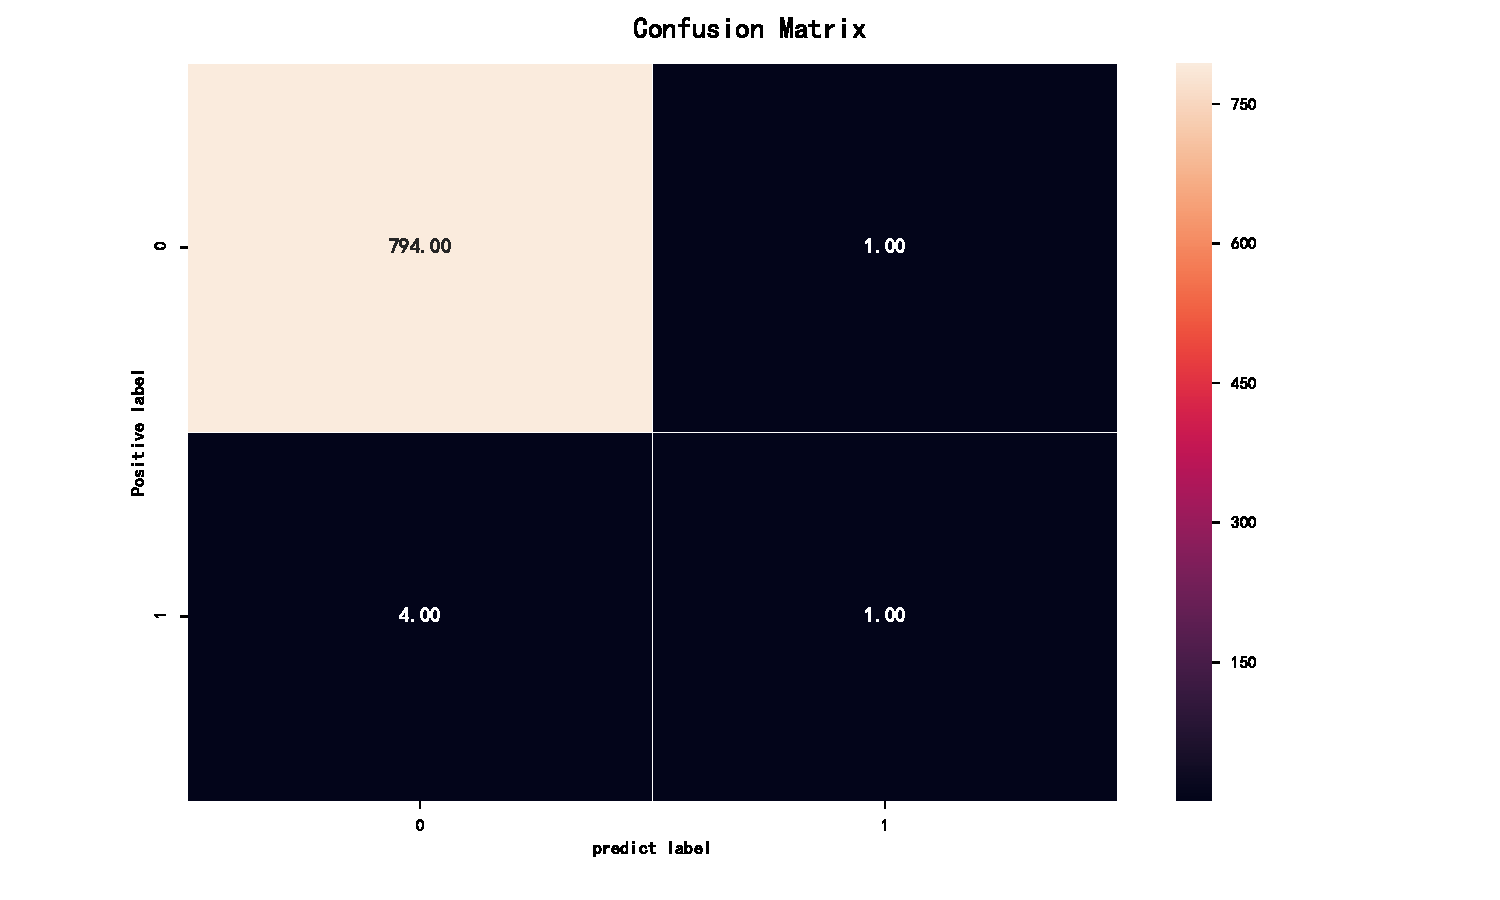
\includegraphics[width=10cm]{./pictures/xgb_CM.pdf}
	\caption{Confusion Matrix of Xgboost classifier}\label{xgb_CM}
\end{figure}
% Table generated by Excel2LaTeX from sheet 'Sheet1'
\begin{table}[htbp]
	\centering
	\caption{Positive predictions of Xgboost classifier}
    \begin{tabular}{ll}
		\toprule
		GlobalID & Possbility \\
		\midrule
		{076DEDA1-899E-4FED-AB26-16FDC985985D} & 0.583 \\
		\rowcolor{mygray}
		{11EDE286-85BA-4433-8AF2-7F60CF8D7409} & 0.532 \\
		{141066CC-E400-401B-A5A3-976BE391849C} & 0.526 \\
		\rowcolor{mygray}
		{19314731-2AAD-4F4E-B425-EF03601A51A7} & 0.732 \\
		{1B4BD010-A445-4190-9B9D-6B81889B4C7A} & 0.535 \\
		\bottomrule
		\end{tabular}%
	\label{tab:Positive_predictions}%
  \end{table}%
  
  
For a binary classifier, the XGBoost model performs poorly. This is mainly because the sample data are too unbalanced. As the positive sample is too sparse, it is difficult for the model to learn effective information about the data distribution of positive example. In addition, the model has a large number of missing values. There are many samples that are missing one or more of the eyewitness notes, lab comments and images.

Xgboost is already a very complex model for binary classification tasks. So until we have more effective data, it is very difficult to improve model performance by tuning the model itself.

Due to the poor performance of our report prediction model, we do not use it to modify the species distribution function and use the version independent of unverified report prediction given by \textbf{Equation \ref{mu1}}. 


\subsection{Priority Level of Unverified Reports}
We measures the priority level of a unverified report $i$ by following 2 principle. 
\begin{itemize}
	\item The more uncertain we are about $\mu(X_i, t_i)$, the higher the priority.
	\item According to information attached toreport $i$, the more likely that report $i$ is a positive sample, the higher the priority.
\end{itemize}

The probability of report $i$ being positive is $p_i=p(Image_i, Note_i, LabComment_i)$. Therefore, we measure the priority of unverified report $i$ by
\begin{equation}
	\varrho_i = \sigma_i(X) \cdot p_i
	\label{priority}
\end{equation}

\subsection{Eradicated Evidence}
We define the eradication of hornets as the maximum value of $\mu_i(X)$ is smaller than a certain threshold $T$: 
\begin{equation}
	\max_X{\mu_i(X)} < T.
\end{equation}
In the current time window, newly received negative samples can reduce the value of the distribution function.And positive samples can dramatically increase the value of the distribution function around them. If no new reports are received within a period of time.The half-life of the distribution function can be given by the number of time Windows according to

\begin{equation}
	halfLife = \frac{\ln 2}{\ln{\frac{w+1}{w}} }.
\end{equation}

\section{Senitivity Analysis}\label{condition}
Sensitivity analysis is a method to study and analyze the sensitivity degree of model state or output change to system parameters or surrounding conditions change
In this section we choose some manually given important parameters and analyze the effects of changing these parameters on the model performance.

\subsection{Sensitivity of $\mu_i(X)$'s AUC to parameter $\gamma$}
According to \textbf{Equation \ref{gamma}}, $\gamma$ determines how fast a sample's contribution to the surrounding density decays with distance. It will affect the density distribution prediction of species $\hat{f}_i(X)$ , and then affect the hornets' relative density distribution $\mu_i(X)$ which stands for the probability of a report at position $X$ to be positive output by our model. 

\begin{figure}[H]%\usepackage{float}
	\small
	\centering
	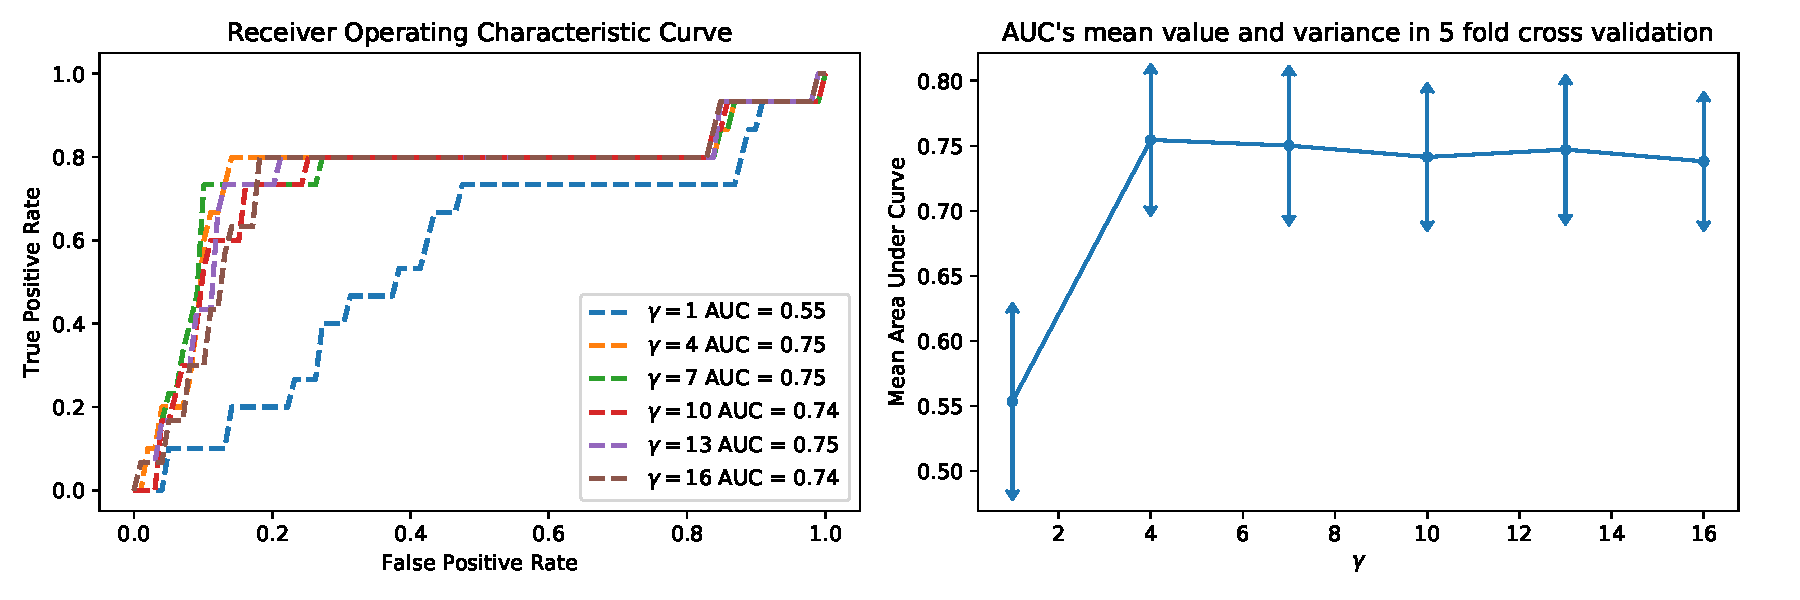
\includegraphics[width=17cm]{./pictures/mean_roc_auc_by_gamma.pdf}
	\caption{Sensitivity of AUC to parameter $\gamma$}\label{mean_roc_auc_by_gamma}
\end{figure}
Our analysis results is shown in \textbf{Figure \ref{mean_roc_auc_by_gamma}}. According to the analysis, as long as $\gamma$ is not too small, the performance of our model $\mu_i(X)$ is stable.

\subsection{Sensitivity of EfficientNet Metrics }
\subsubsection{Image filter threshold $p_t$}
Because we only use images of quality above a certain threshold for training.The threshold of image filtering will affect the performance of the model.If the threshold is too high, the training set will be too small, and CNN cannot obtain enough data for training.If the threshold is too low, the image data set will have too much noise, which is not conducive to the learning and convergence of the network.

\begin{figure}[H]%\usepackage{float}
	\small
	\centering
	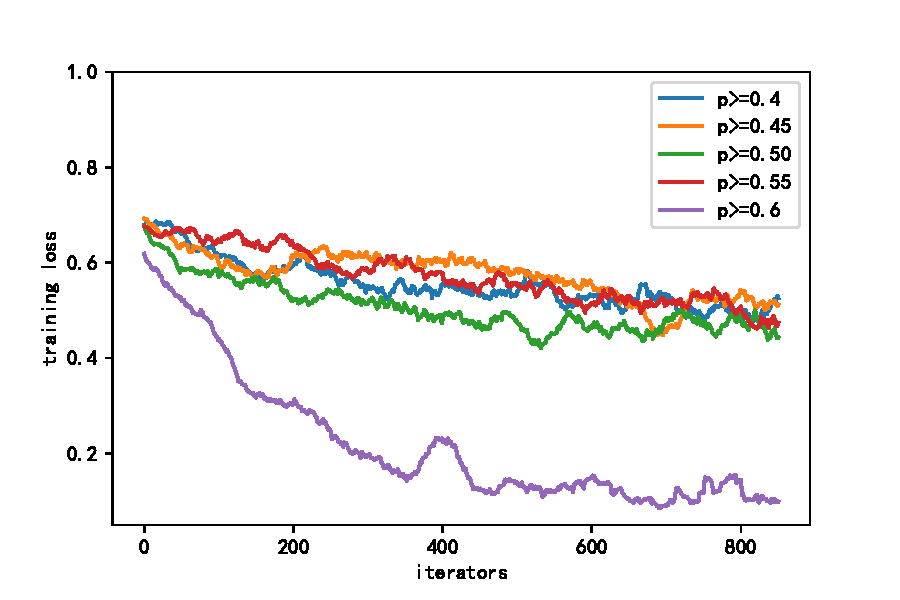
\includegraphics[width=8.5cm]{./pictures/loss2.pdf}
	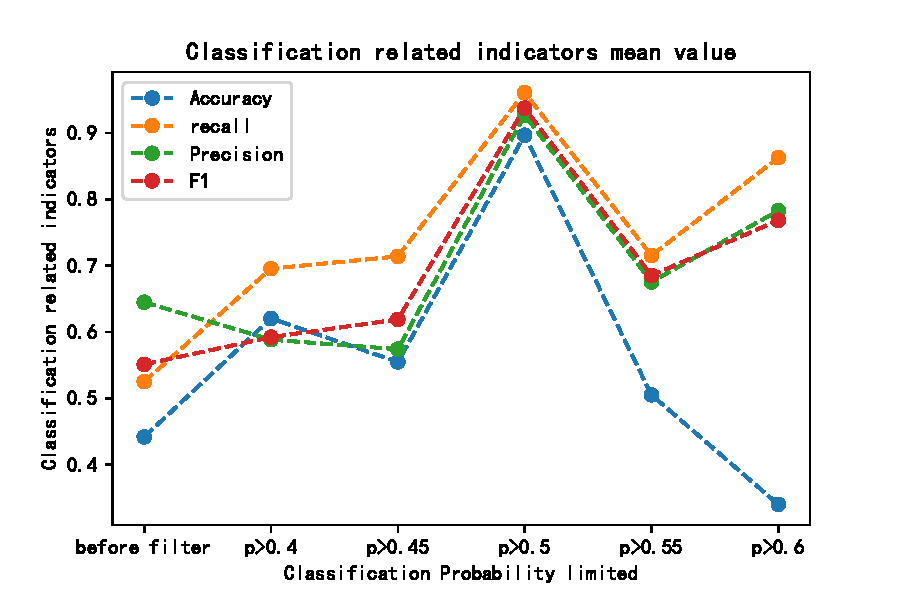
\includegraphics[width=8.5cm]{./pictures/acc.pdf}
	\caption{Training Loss and mean value of Metrics in best fold}\label{loss_acc_sensitivity}
\end{figure}
\textbf{Figure \ref{loss_acc_sensitivity}} shows the training process and final metrics of the model under different image filtering thresholds. We can see $p_t$ have a great influence on the performance of Efficientnet.The performance of the model reached the highest at at $p_t=0.5$.

\subsubsection{Number of folds in the cross-validation $k$}
Due to insufficient sample data of image data set, different cross-validation sampling may lead to deviation of data distribution, thus affecting model performance. \textbf{Figure \ref{kfold_sensitivity}} shows the final loss of the model in different cross-validation.
\begin{figure}[H]%\usepackage{float}
	\small
	\centering
	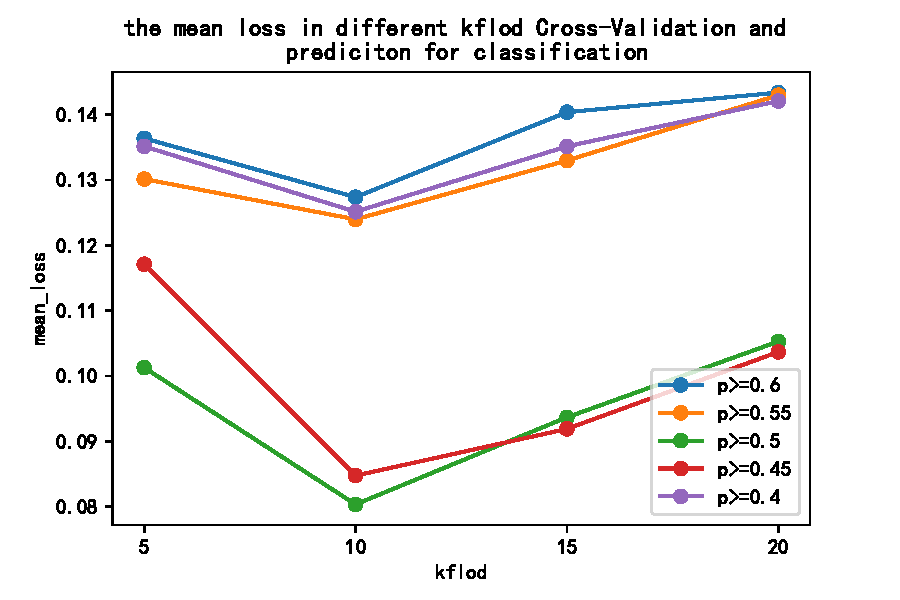
\includegraphics[width=10cm]{./pictures/kfold_Sensitivity.pdf}
	\caption{Training Loss and mean value of Metrics in best fold}\label{kfold_sensitivity}
\end{figure}
We can find that $k$ does not have a big influence on the performance of the model, and roughly the best performance is achieved when $k=10$.


\section{Strengths and Weaknesses}
\subsection{Strengths}
\begin{itemize}
	\item Our species relative density estimation model uses a continuous kernel density estimation algorithm. It doesn't depend on meshing the space. There is only one parameter $\gamma$ needs to be specified manually. Moreover, it can be proved that the performance of the model is stable relative to $\gamma$ within a wild range.
	\item We use an open source pretrained model to filter the image data set. It can be proved that image filtering greatly improves the performance of the classification model.
	\item We did our best to consider all the data available to us. Our binary classifier for unverified witness report takes into account the output of the image classifier, description from the witness, laboratory comments and the seasonal habits of hornets.
	\item Our model can be easily implemented if more detailed geographic data and report information is available which shows a strong robustness.
\end{itemize}
\subsection{Weaknesses}
\begin{itemize}
	\item Our species density estimation model can not give an accurate estimate of species density for areas with sparse reports.
	\item For eyewitness's description, as well as laboratory comments, we only utilize simple features through regular matching and output  of natural language sentiment classification model. We didn't dig deeper into information in the text and compare it with the real features of hornet.
\end{itemize}

\section{conclusion}
In our proposal, we describe the spread of hornet by \textbf{species relative density distribution} $\mu_i(X)$ which is the possibility of a report to be positive in the ith time window at location $X$. $\mu_i(X)$ is obtained by \textbf{species density function} estimated by \textbf{KDE-method}. In order to synthesize the historical distribution and report information in the current time window, $\mu_i(X)$ is updated by \textbf{Equation \ref{nu_update}}.

A credibility estimation model for undetected reports $p_i$ can not only be used to rank the priority of unverified reports, but also enable us to use  unverified reports to modify hornets' relative density distribution function $\mu_i(X)$. \textbf{EfficientNet} is an image classifier. Given the image, it outputs a confidence probability measure of the likelihood that the image is a hornet. NLP is a \textbf{emotion classification model} based on natural language processing , whose input is the expert's evaluation of the report, and output a positive emotion intensity to measure the expert's attitude towards the report. The two features above, along with other features extracted from the report data, such as season information and whether the report provides bee length, are extracted as features. All these features are fed into the machine learning model which give the results of \textbf{Unverified Report Prediction}. 

The denser the reported samples is near location $X$, the lower the uncertainty of the model's prediction. The uncertainty level of the prediction at location $X$ is given by \textbf{Equation \ref{uncertainty}}. The \textbf{unverified report priority} given by \textbf{Equation \ref{priority}} takes both its credibility and uncertainty level of our model at position $X$ into account.

We define that the hornet species have disappeared in this area if the maximum value of the distribution function is less than threshold $T$ which can be interpreted as the maximum proportion of hornets in all bees is negligible.

So far, our hornet species distribution model based on \textbf{KDE} density estimation has been completely established.

\clearpage
%我们对于您的地区受到大黄蜂物种入侵的困扰深感抱歉。我们相信您与我们一样意识到了大黄蜂对于当地物种以及居民人身安全所可能产生的严重影响。
\section*{Memo}\addcontentsline{toc}{section}{Memo}

\begin{flushleft}
	%Dear senator from Washington State:
	The Washington State Department of Agriculture:
\end{flushleft}

Thank you very much for your time. We are sorry that your area has been plagued by an invasion of hornets species. We believe that you have fully awared of the serious impact that hornets can have on the safety of local species and resident. We share your urgency to address hornets invasion problem.

%我们的物种入侵监测系统致力于利用目击报告中一切可用的信息。得出对于定大黄蜂物种的分布和传播情况进行一个直观的统计和预测。我们的模型基于可靠的数学原理,利用了最先进的深度卷积神经网络以及自然语言情感分类模型并且针对性考虑了蜜蜂的习性。
Our hornet species invasion surveillance system is based on species density estimation algorithm. It aims to use all available information from eyewitness' reports. Our model can predict and visualize the distribution and spread of hornet species. It is based on sound mathematical principles and uses the state of the art deep convolutional neural network structure and natural language emotion classification model. Also the unique behavior and living habits of hornets is taken into account.

we have some suggestions for you:
\begin{enumerate}[\bf 1.]
	%我们希望您鼓励居民对于目击事件进行可靠的观察和报告。包括清晰展现蜜蜂细节的照片(视频)以及对于蜜蜂特征的详尽描述。甚至可以对得到验证的高质量报告进行经济奖励。
	\item We suggest you to encourage local residents to make as much reliable observations and reports as possible. Includes photos (videos) that \textbf{show bees' detailed feature and descriptions of their characteristics}. There can even be financial rewards for verified, high-quality reports.
	%我们希望您调集尽可能多的政府资源来验证目击报告,因为更多被验证的目击报告能够使得监测模型对于黄蜂分布的预测更加准确。如果实际操作中可用的资源不足以验证所有的目击报告,那么我们强烈建议您根据模型给出的优先级顺序来优先验证目击报告。我们的优先级顺序综合考虑了报告的可信度以及目击位置当前模型预测分布情况的不确定性。
	\item We suggest you to mobilize as many government resources as possible to verify sighting reports, because more verified reports will make the species distribution model's prediction more accurate. If in practice the resources available are not enough to validate all sightings, we strongly recommend that you \textbf{prioritize sightings according to the priority level given by the model}. Our prioritization takes into account both the reliability of the reports and the uncertainty of the distribution of current model predictions of sighting locations.
	%我们建议回复居民报告的专家在用语言回复的同时对于报告的可信度给出一个打分。我们意识到了人力资源是最昂贵的资源。但是一方面目前的机器学习算法仍然不能完全替代人类专家的经验。另一方面既然专家已经给出了评论,就说明他对于现有的信息的可信度已经做出了一个评估。所以进行一个数值上的打分并不会大幅提高专家的工作量,但是如果考虑了人类专家的意见机器学习算法预测的准确性会大幅度提升。
	\item We recommend that \textbf{experts who comment to residents' reports give a score on the reliability of the report} as well as their message responses. We realize that human resources are the most expensive resources. But on one hand the current machine learning algorithms are still unable to completely replace the experience of human experts. On the other hand, since the expert has commented, he or she must has made an assessment of the credibility using available information. Therefore, giving a numerical score will not dramatically increase the workload of experts, but the accuracy of machine learning algorithm prediction will be greatly improved if the opinions of human experts are taken into account.
	%我们希望能获取到详细的华盛顿州地理数据,包括但不限于海拔高度,森林覆盖密度,降雨量和月平均气温。以及当地物种的分布统计数据。目前我们的模型对于物种密度的预测值考虑了经度和纬度两个地理特征。这些特征都可能影响大黄蜂在该地区的宜居程度,所有如果我们获得了更详细的地理特征数据,模型必然会给出更精确的预测结果。此外,黄蜂的分布会与当地物种的分布相互作用。比如说大黄蜂在9月和10月会大幅猎杀其他蜜蜂。日本蜜蜂(Apis cerana japonica)与亚洲大黄蜂共同进化,对它们有防御能力。
	\item We would like to obtain \textbf{detailed geographic data for the state of Washington} (including but not limited to elevation, forest cover density, rainfall and monthly mean temperature) and statistics on the distribution of local species.  All of these features may affect the habitability of bumblebees in the region, but at present, our model's prediction of species density only considers longitude and latitude. If we get more detailed geographical data, the model is bound to give more accurate predictions. In addition, the distribution of hornets can interact with local species. For example, hornets hunt down other bees in September and October. The Japanese honey bees (Apis cerana japonica) coevolved with the Asian bumblebee and is defensible against it.
	%我们建议您加大对大黄蜂生活习性的宣传。一方面,这可以提高报告的质量,减少误报的比例。现在大部分的目击报告都是误报。由于样本的不均衡,模型的效果也会受到影响。另一方面,减少误报的比例,可以节约政府的调查资源,使得更多有价值的目击报告可以被验证。此外,对大黄蜂的了解可以提高居民的自我保护意识,减少可能的人员受伤和经济损失。
	\item We suggest that you \textbf{increase the publicity of hornet knowledge} such as its appearance and living habits. On one hand, this can improve the quality of the report and reduce the proportion of negative report. At present, most sightings are negative. Due to the imbalance of samples, the model's performance is also affected. On the other hand, reducing the rate of false positives could save the government's investigative resources and allow more valuable eyewitness reports to be verified. In addition, the understanding of hornet can improve residents' awareness of self-protection and reduce possible human injuries and economic losses.
\end{enumerate}
We sincerely hope that the problem of hornet species invasion can be solved as soon as possible so that you and local residents will not be bothered by it anymore.
\clearpage
\begin{thebibliography}{99}
	\addcontentsline{toc}{section}{References}  %引用部分标题("Refenrence")的重命名
	\bibitem{1}Hwang, Jenq-Neng, Shyh-Rong Lay, and Alan Lippman. "Nonparametric multivariate density estimation: a comparative study." IEEE Transactions on Signal Processing 42.10 (1994): 2795-2810.
	\bibitem{GLMs}Guisan, Antoine, Thomas C. Edwards Jr, and Trevor Hastie. "Generalized linear and generalized additive models in studies of species distributions: setting the scene." Ecological modelling 157.2-3 (2002): 89-100.
	\bibitem{Bayesian} ASPINALL, RICHARD. "An inductive modelling procedure based on Bayes' theorem for analysis of pattern in spatial data." International Journal of Geographical Information Systems 6.2 (1992): 105-121.
	\bibitem{Ecological‐niche}Hirzel, Alexandre H., et al. "Ecological‐niche factor analysis: how to compute habitat‐suitability maps without absence data?." Ecology 83.7 (2002): 2027-2036.
	\bibitem{2}Phillips, Steven J., Robert P. Anderson, and Robert E. Schapire. "Maximum entropy modeling of species geographic distributions." Ecological modelling 190.3-4 (2006): 231-259.
	\bibitem{roc}Hanley, James A., and Barbara J. McNeil. "The meaning and use of the area under a receiver operating characteristic (ROC) curve." Radiology 143.1 (1982): 29-36.
	\bibitem{Imagenet}Deng, Jia, et al. "Imagenet: A large-scale hierarchical image database." 2009 IEEE conference on computer vision and pattern recognition. Ieee, 2009.
	\bibitem{EfficientNet}Tan, Mingxing, and Quoc Le. "Efficientnet: Rethinking model scaling for convolutional neural networks." International Conference on Machine Learning. PMLR, 2019.
	\bibitem{focal_loss}Mukhoti, Jishnu, et al. "Calibrating deep neural networks using focal loss." arXiv preprint arXiv:2002.09437 (2020).
	\bibitem{k_fold_cv}Bengio, Yoshua, and Yves Grandvalet. "No unbiased estimator of the variance of k-fold cross-validation." Journal of machine learning research 5.Sep (2004): 1089-1105.
	\bibitem{sentiment_analysis}Araci, Dogu. "Finbert: Financial sentiment analysis with pre-trained language models." arXiv preprint arXiv:1908.10063 (2019).
	\bibitem{BERT}Devlin, Jacob, et al. "Bert: Pre-training of deep bidirectional transformers for language understanding." arXiv preprint arXiv:1810.04805 (2018).
	\bibitem{Xgboost}Chen, Tianqi, and Carlos Guestrin. "Xgboost: A scalable tree boosting system." Proceedings of the 22nd acm sigkdd international conference on knowledge discovery and data mining. 2016.
\end{thebibliography}

\clearpage

% \section*{Appendices}\addcontentsline{toc}{section}{Appendices}
% 	\noindent Appendix1:
% 	%下面的是配置是可以写中文注释的python环境:
% 	%\usepackage{listings}
% 	%\usepackage{color}
% 	\definecolor{dkgreen}{rgb}{0,0.6,0}
% 	\definecolor{gray}{rgb}{0.5,0.5,0.5}
% 	\definecolor{mauve}{rgb}{0.58,0,0.82}
% 	\lstset{	frame=shadowbox,                           % shadowbox framed
% 		rulesepcolor= \color{gray},%框的颜色
% 		language=Python,
% 		aboveskip=3mm,
% 		belowskip=3mm,
% 		showstringspaces=false,
% 		columns=flexible,
% 		basicstyle={\small\ttfamily},
% 		numbers=left,%设置行号位置none不显示行号
% 		%numberstyle=\tiny\courier, %设置行号大小  
% 		numberstyle=\tiny\color{gray},
% 		keywordstyle=\color{blue},
% 		commentstyle=\color{dkgreen},
% 		stringstyle=\color{mauve},
% 		breaklines=true,
% 		breakatwhitespace=true,
% 		escapeinside=``,%逃逸字符(1左面的键),用于显示中文例如在代码中`中文...`
% 		tabsize=4,
% 		extendedchars=false %解决代码跨页时,章节标题,页眉等汉字不显示的问题  
% 	}
% \begin{lstlisting}
% from sklearn.svm import SVC
% classifier = SVC(kernel = 'rbf',C=0.8, random_state = 0,class_weight={0:20,1:24})
% #classifier = SVC(kernel = 'rbf',C=1.2, random_state = 0)
% classifier.fit(X_train, y_train)
% # Predicting the Test set results
% y_pred = classifier.predict(X_test)

% \end{lstlisting}
	
	

%%%%%%%%%%%%%%%%%%%%%%%%%%%%%%
\end{document}
